\documentclass[]{uc2pfecaneva}


% Title Page
\title{}
\author{}


\begin{document}
	\setlength{\parskip}{6pts}

	\tableofcontents
	\listoffigures
	\listoftables
\chapter{Analysis}

\newpage

\raggedright\section{Introduction}
\paragraph{}
	The analysis phase of the development process of any system is crucial, since any specifications in this part will heavily impact the system's behaviour, functionality, and interactions.
\paragraph{}
	We will focus in this chapter on analysing the requirements for our system, as well as establishing its boundaries, starting with the project context, triggers, problematic, and objectives. The following step is identifying the actors of the system and their roles. Next, we will address the functional and nonfunctional requirements. Following that, we will specify the static context diagram and the use case diagram for each actor individually, then the global use case diagram. The final step will be to choose five use cases from which to develop their descriptive sheet, system sequence diagram, and prototypes for Human-Computer Interaction, along with a conclusion.

\raggedright\section{Specifications (Cahier Des Charges)}
\subsection{Project context}
\paragraph{}
	During the period of the CoVid-19 pandemic, On-Site examinations were not allowed for health reasons, this, combined with the fact that the nature of our education as software engineers demands us to use smart devices all the time, all these factors suggested and triggered the need of an online examination system.
\paragraph{}
	In this system, students can take online exams instead of in-person exams, teachers create and proctor exams, and administrators manage all those things. At the same time, we ensure that the examinations are secure and in great measure as well.

\subsection{Problematic and project limitations}
	\subsubsection{Problematic}

	\begin{itemize}
		\item How to protect the system from most online attacks (injections, DDoS attacks, etc..).
		\item How to prevent students from using any type of cheats.
		\item How to make a strict examination system yet doesn't ruin the examinator experience.
		\item How to take advantage of artificial intelligent technics to boost the system’s efficiency and help the proctor.
		\item How to include automatic exam evaluation.
		\item How to make a robust system that stands against unexpected scenarios: server getting down, data loses, etc.
\end{itemize}


	\subsubsection{project limitations}

	\begin{itemize}
		\item The system won't manage and organize students and teachers because it's an examination system and not a school management system.
		\item Each instance of the system is Linked to a single school or university, which means the system is only interested in examining students of that school, any examinee that doesn't study at that school can’t use the system.
		\item The System won't be interested in examining Non-scholars.
	\end{itemize}


\subsection{Project objective}



\raggedright\section{Identification of actors}
\raggedright\subsection{Admin}
\paragraph{}
	The administrator is an employee of the university administration. He or she is responsible for all collective administrative tasks that need to be performed in the system.

\raggedright\subsection{Head Teacher}
\paragraph{}
	The head teacher is the main teacher of the module in the university, whose role is to create questions and exams, as well as to evaluate the students' answers.

\raggedright\subsection{Teacher TD/TP}
\paragraph{}
	Teacher of TD (tutorials) / TP (practical work) is the person who is responsible for creating questions and evaluating student responses


\raggedright\subsection{Student}
\paragraph{}
	The student is the individual who enrolled at a university; it is he who passes exams and consults the results of a specific course on the system.

\raggedright\subsection{Proctor}
\paragraph{}
	Proctor is a university teacher who is assigned to proctor the students at exams and to conduct exam-related activities such as ensuring the real students are present, starting the exam, and supervising it.

\raggedright\section{Non Functional Requirements}
\raggedright\subsection{Admin}
\begin{itemize}
\item The admin cant see the exam questions.
\item When assigning modules to teachers, the admin should choose the teacher’s type (responsible of module, Tp/Td).
\item When assigning proctors to an exam session, the admin should give the proctor his privileges (can start/end exam session, can kick student, etc...).
\item When adding a student or a teacher, the admin can generate a password for the user to be used for his first login.
\item The admin is the responsible of specifying the exam date.
\item Should save backups for the system’s database and configuration once in a while, to able to restore the system’s state when  unexpected problems acure .

\end{itemize}

\raggedright\subsection{Head Teacher}
\begin{itemize}
	\item Can only see modules that are assigned to him by admin.
	\item The question bank is created automatically every new academic year.
	\item Previous question banks are available.
	\item Can’t create or delete any question bank.
	\item Can only delete questions made by him.
	\item When creating an exam, there is an option for an auto-evaluated exam, where he must provide answers for each question.
	\item Can’t create an exam with no questions.
	\item Can’t modify published exams.
	\item Can’t search for students responses by their names.
\end{itemize}

\raggedright\subsection{Teacher TD/TP}
\begin{itemize}
	\item Can’t create exams.
	\item Can only consulate/modify/delete his own questions.
	\item When he evaluates a student’s response it can be changed by the teacher responsible of module.
\end{itemize}

\raggedright\subsection{Student}
\begin{itemize}
	\item Can only see exams that are assigned to him by the admin.
	\item Can either see a list view or a calendar view for his exams.
	\item The Student’s computer, operating system and internet  must satisfy the minimal requirements test for him to be allowed to take exams.
	\item The  minimal requirements test is available any time.
	\item The Student can communicate with the proctor.
	\item The communication is limited.
	\item Can leave the exam session only if the leaving option is activated by the proctor or the exam duration is finished.
	\item Can give feedback about the exam.
	\item Can see his exam mark and the mark for each question.
	\item When consulting exam results, he can see the correct answers for his mistakes.
\end{itemize}

\raggedright\subsection{Proctor}
\begin{itemize}
\item Can’t start an exam session if the number of students is less than the minimum number specified by the admin.
\item When a proctor leaves a comment an specific student, only proctors from the same room will be able to see it.
\item When writing a public message, it can be sent either to all students or all proctors.
\item Can only kick students from the room he is assigned to.
\item After kicking a student, a report to explain the reason of kicking is necessary.
\end{itemize}


\raggedright\subsection{System}

\raggedright\subsubsection{Security}
\begin{itemize}
	\item Role based access.
	\item 2 step verification (confirmation by email or SmS) for all user types (admin , teacher, proctor, student).
	\item Users must enter their password before changing their profile.
	\item The users can't use weak passwords.
	\item Users passwords will be hashed before being stored in the database.
	\item Web-Socket communication between the client app and the server must be encrypted.
	\item When a new user account is created (admin, student, teacher), the system generates a password for the user to be used for his first login, this password must be changed.
	\item The system should be immune to any type of injections.
	\item The students won’t pass exams on the browser, instead they need to download a Desktop app for better security and monitoring.
	\item The Desktop application must be immune to any type of screen recording and camera recording.
	\item The desktop client server is completely separated from the main server for better security and to prevent both servers getting infected when one of them is hacked .
\end{itemize}

\raggedright\subsubsection{Performance}
\begin{itemize}
	\item The system should be able to handle a large amount of student at the same time.
	\item The response time of the server is critical especially in exam sessions.
	\item The desktop client does not communicate to the main server, instead it communicates with its own server for better performance and short response time even when the main server is falling behind.
\end{itemize}

\raggedright\subsubsection{Robustness and Reliability}
\begin{itemize}
	\item The admin can save backups of the system’s database and configuration any time, to able to restore the system’s state when  unexpected problems acure .
	\item Another reason to have two servers instead of one is to avoid getting the whole server down, so we insure that by separating it .
\end{itemize}

\raggedright\subsubsection{Data integrity}
\begin{itemize}
	\item The system will save all conversations between students an proctors.
	\item The system will save all session webcam records.
	\item Deleted teachers, students are saved in the history.
	\item Keep logs of users activities and system’s exceptions.
	\item When students are taking an exam, the system will save their answers automatically every 30 seconds.
\end{itemize}

\raggedright\subsubsection{Portability}
\begin{itemize}
	\item The main system is available through the browser so it can be accessed from any device.
	\item The students can pass exams on any desktop platform (Windows, Linux, macOs).
\end{itemize}

\raggedright\subsubsection{Privacy and Confidentiality}
\begin{itemize}
	\item Student can only see his own marks not other students maks.
	\item The admin can’t see exams or questions.
	\item Saved conversations and webcam records can only be checked by the teacher, also they cant be downloaded or saved.
	\item All saved conversations and webcam records will be deleted automatically when a new semester starts.
\end{itemize}
\raggedright\section{Use-case diagrams}
\subsection{Global use-case diagram}

     \begin{figure}[ht]
	
	\centering
	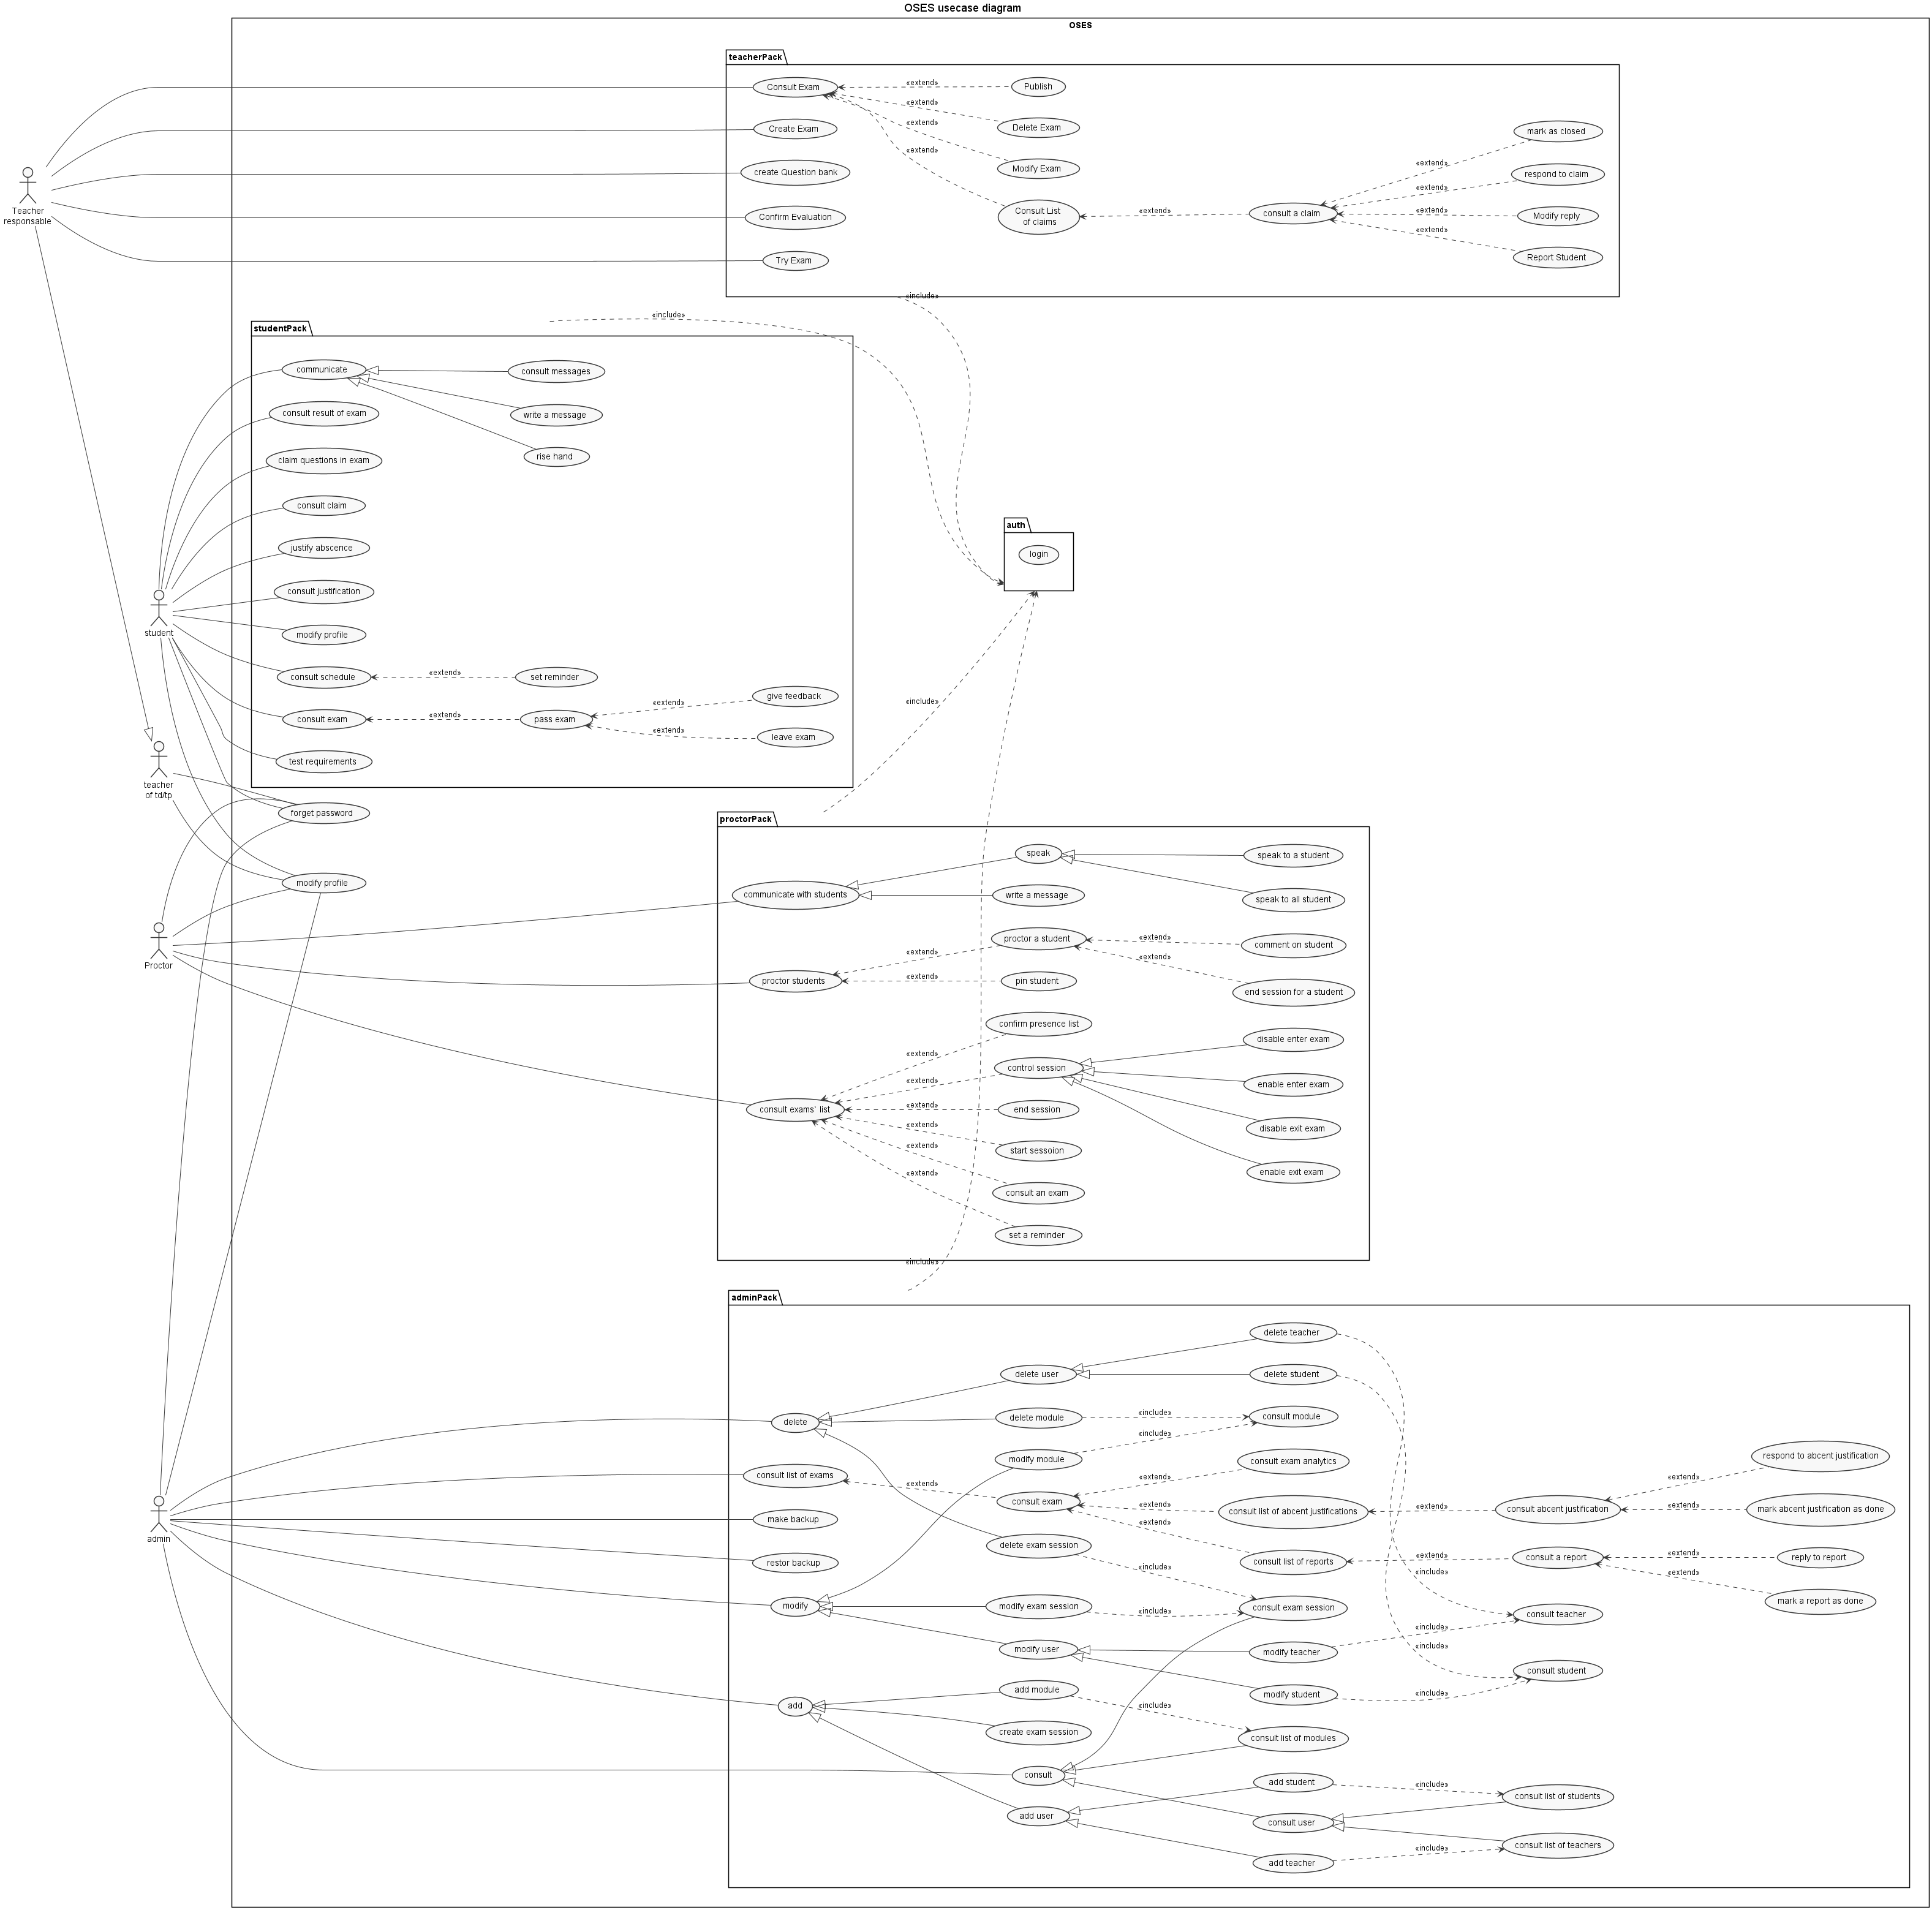
\includegraphics[width=\textwidth]{images/GUCD}
	
	\caption{Global use-case diagram.}
	\end{figure}
\clearpage


\begin{table}[h]
	\raggedright\section{Specifications for 5 Use-cases}

	\raggedright\subsection{Use Case: Login}
	\subsubsection{Descriptive sheet}
	\centering
	\begin{tabularx}{\textwidth}{|l|X|}
		\hline
		Use case name         & login                                                                                                                                                                \\ \hline
		Type                  & principal                                                                                                                                                            \\ \hline
		Actors                & admin, head teacher, teacher td/tp, student, proctor                                                                                                                 \\ \hline
		Objective             & Authenticate the user who tries to access to the platform                                                                                                            \\ \hline
		Preconditions         &                                                                                                                                                                      \\ \hline
		nominal scenario
		                      & 1) The user enter his email and password.                                                                                                                            \\
		                      & 2) The system verifies the information.                                                                                                                              \\
		                      & 3) The System asks user where he wants to receive his verification code.                                                                                             \\
		                      & 4) The user chooses verification by email.                                                                                                                           \\
		                      & 5) the System sends a verification code to the user's email.                                                                                                         \\
		                      & 6) the System asks the user to enter his verification code.                                                                                                          \\
		                      & 7) the user enters the code and clicks on "Confirm".                                                                                                                 \\
		                      & 8) the system shows a success message.                                                                                                                               \\ \hline
		Alternative scenarios
		                      & A1 : User chooses verification by SMS,  Sequence can start after the point 3 of the nominal scenario.                                                                \\
		                      & \hspace{4mm}3.1) The user chooses verification by SMS.                                                                                                               \\
		                      & \hspace{4mm}3.2) the System sends a verification code to the user's phone number.                                                                                    \\
		                      & \hspace{4mm}3.3) the System asks the user to enter his verification code.                                                                                            \\
		                      & \hspace{4mm}3.4) the user enters the code and clicks on "Confirm".                                                                                                   \\
		                      & \hspace{4mm}3.5) the system shows a success message and redirects the user to the home page.                                                                         \\ \hline
		Exception scenarios
		                      & E1 : User enters a wrong email or password: Sequence can start after the point 2 of the nominal scenario.                                                            \\
		                      & \hspace{4mm}2.1) The system shows an error message "wrong email or password".                                                                                        \\
		                      & \hspace{4mm}2.2) The nominal scenario                                                                                                                                \\
		                      & E2 : User enters a expired or invalid verification code: Sequence can start after the point 7 of the nominal scenario.                                               \\
		                      & \hspace{4mm}7.1) The system shows an error message "The verification code is expired or invalid".                                                                    \\
		                      & \hspace{4mm}7.2) The nominal scenario                                                                                                                                \\
		                      & E3 : User enters a wrong password 5 times: Sequence can start after the point 2 of the nominal scenario.                                                             \\
		                      & \hspace{4mm}7.4) The system shows an error message "you entered too many wrong passwords in a short time, please try again later or try clicking (forgot password)". \\
		                      & \hspace{4mm}7.2) The nominal scenario                                                                                                                                \\ \hline
		Post conditions
		                      & The user is authenticated and redirected to the Home page                                                                                                            \\ \hline
	\end{tabularx}
	\caption{Descriptive sheet for the use case: login.}
	\label{table:1}
\end{table}
\clearpage

\subsubsection{system sequence diagram}
     \begin{figure}[h]
	
	\centering
	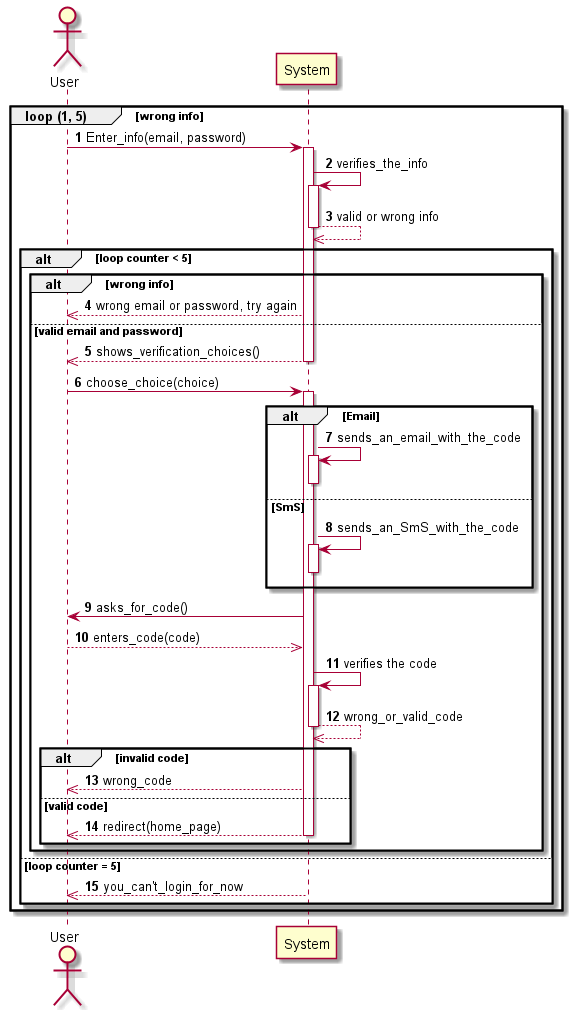
\includegraphics[width=260pt]{images/Login_dss}
	
	\caption{system sequence diagram for the use case: login.}
\end{figure}
\clearpage

\subsubsection{prototypes}
     \begin{figure}[h]
	
	\centering
	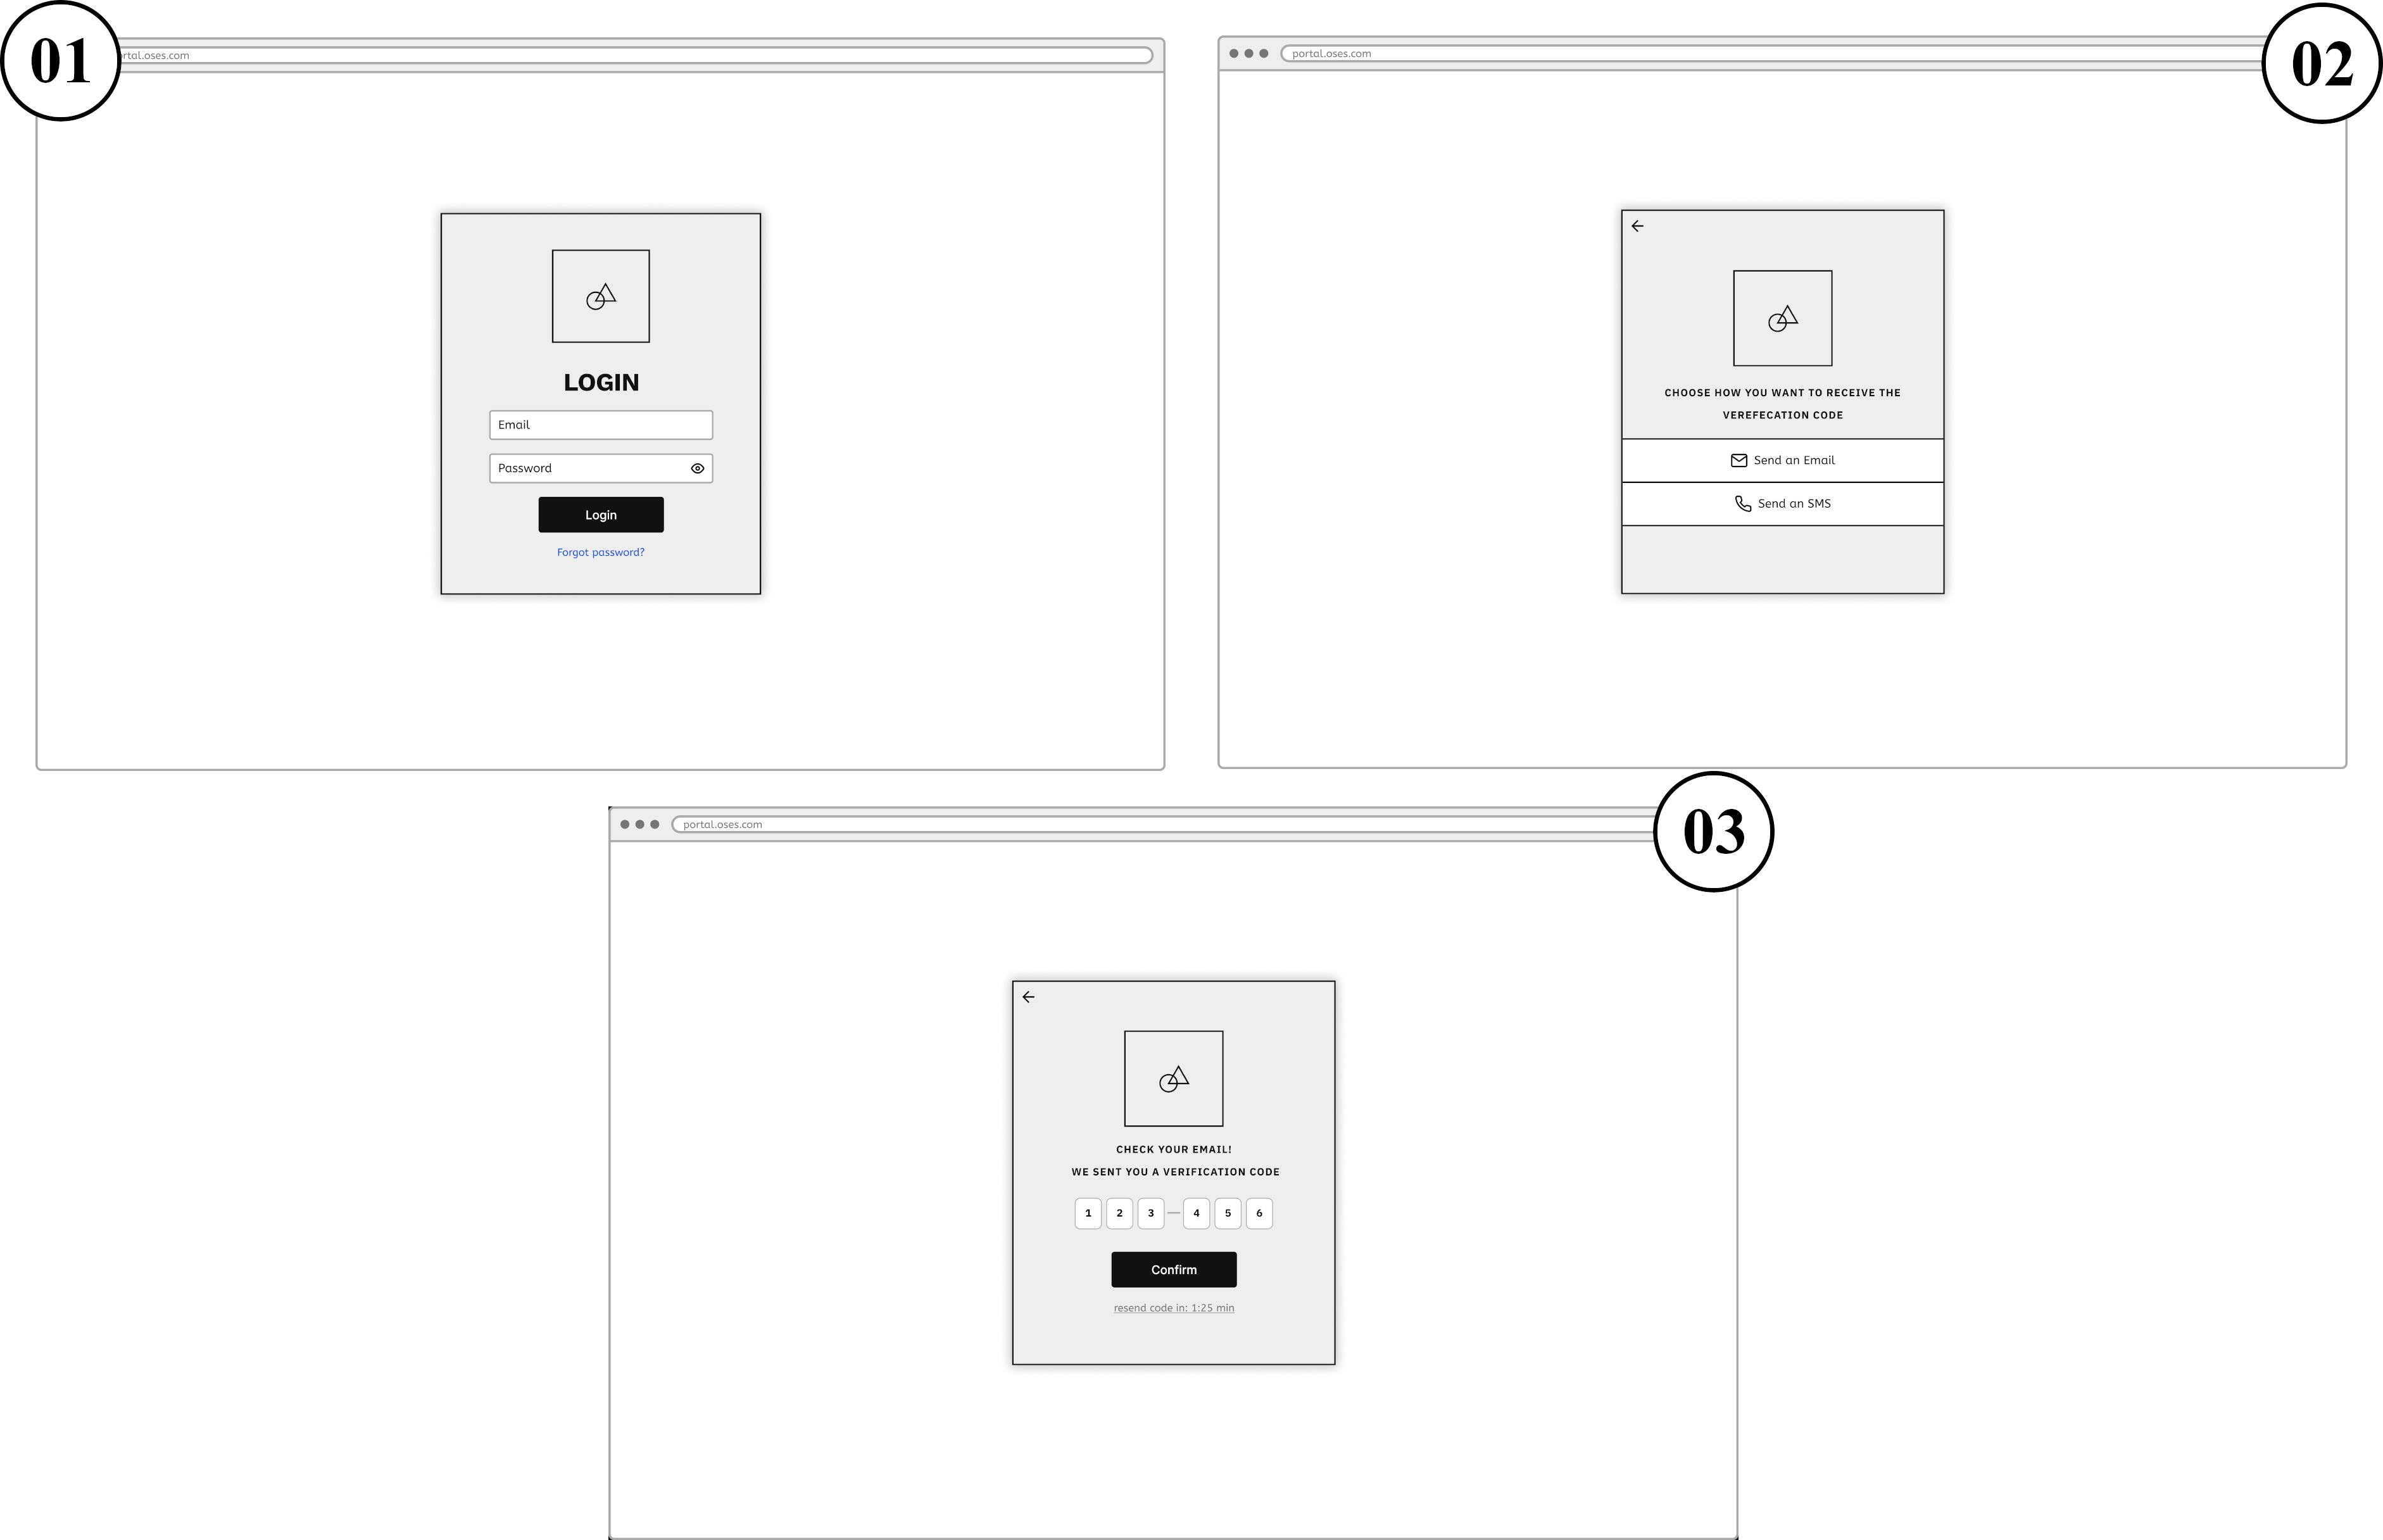
\includegraphics[width=\textwidth]{images/login}
	
	\caption{Prototypes for the use case: login.}
\end{figure}
\clearpage


\begin{table}[t]
	\raggedright\subsection{Use Case: Create an exam session}
	\subsubsection{Descriptive sheet}
	\centering
	\begin{tabularx}{\textwidth}{|l|X|}
		\hline
		Use case name         & Create an exam session                                                                                                                                            \\ \hline
		Type                  & principal                                                                                                                                                         \\ \hline
		Actors                & admin                                                                                                                                                             \\ \hline
		Objective             & create an exam session with time, students and proctors specifications.                                                                                           \\ \hline
		Preconditions         &                                                                                                                                                                   \\
		& - Admin logged in.                                                                                                                                                \\
		& - consulted the list of modules.                                                                                                                                  \\
		& - consulted a module.                                                                                                                                             \\ \hline
		nominal scenario      &                                                                                                                                                                   \\
		& 1) The admin clicks on "create an exam session" button.                                                                                                           \\
		& 2) The system shows a form to be filled by the admin.                                                                                                             \\
		& 3) The admin fills the form.                                                                                                                                      \\
		& 4) The system checks and examines the validation of the filled information.                                                                                       \\
		& 5) The admin clicks on save.                                                                                                                                      \\
		& 6) The system saves the created exam session.                                                                                                                     \\
		& 7) The system notify the admin that the exam is created successfully.                                                                                             \\
		& 8) The system notifies the module 's head teacher about the created exam session.                                                                                 \\
		& 9) Notify the students about the date of the exam session.                                                                                                        \\ \hline
		Alternative scenarios &                                                                                                                                                                   \\
		& A1: Incorrect fields: this scenario starts after step number 4 of scenario nominal.                                                                               \\
		& \hspace{4mm}4.1) The system finds that some fields' information is invalid or the required fields are not filled.                                                 \\
		& \hspace{4mm}4.2) The system highlights the fields with invalid information or the ones that are required with messages of how valid information should look like. \\
		& \hspace{4mm}4.3) The scenario continues from step 3 of the scenario nominal.                                                                                      \\ \hline
		Exception scenarios   &                                                                                                                                                                   \\ \hline
		Post conditions       &                                                                                                                                                                   \\
		& - students Notified about the date of the exam.                                                                                                                   \\
		& - head teacher of the course is notified of the created exam session.                                                                                             \\
		& - an exam session has been created.                                                                                                                               \\ \hline
	\end{tabularx}
	\caption{Descriptive sheet for the use case: create an exam session.}
	\label{table:2}
\end{table}
\clearpage

\subsubsection{system sequence diagram}
\begin{figure}[h]
	
	\centering
	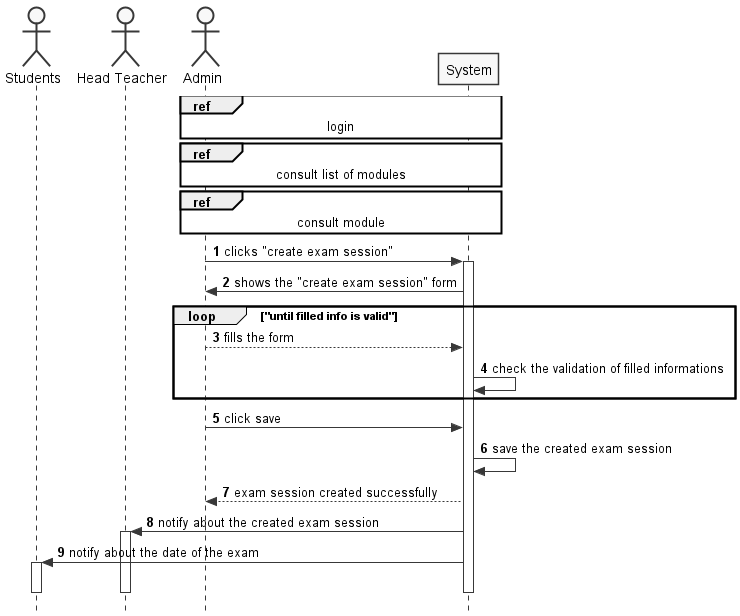
\includegraphics[width=\textwidth]{images/create_exam_session}
	
	\caption{system sequence diagram for the use case: create an exam session.}
\end{figure}
\clearpage

\subsubsection{prototypes}
\begin{figure}[h]
	
	\centering
	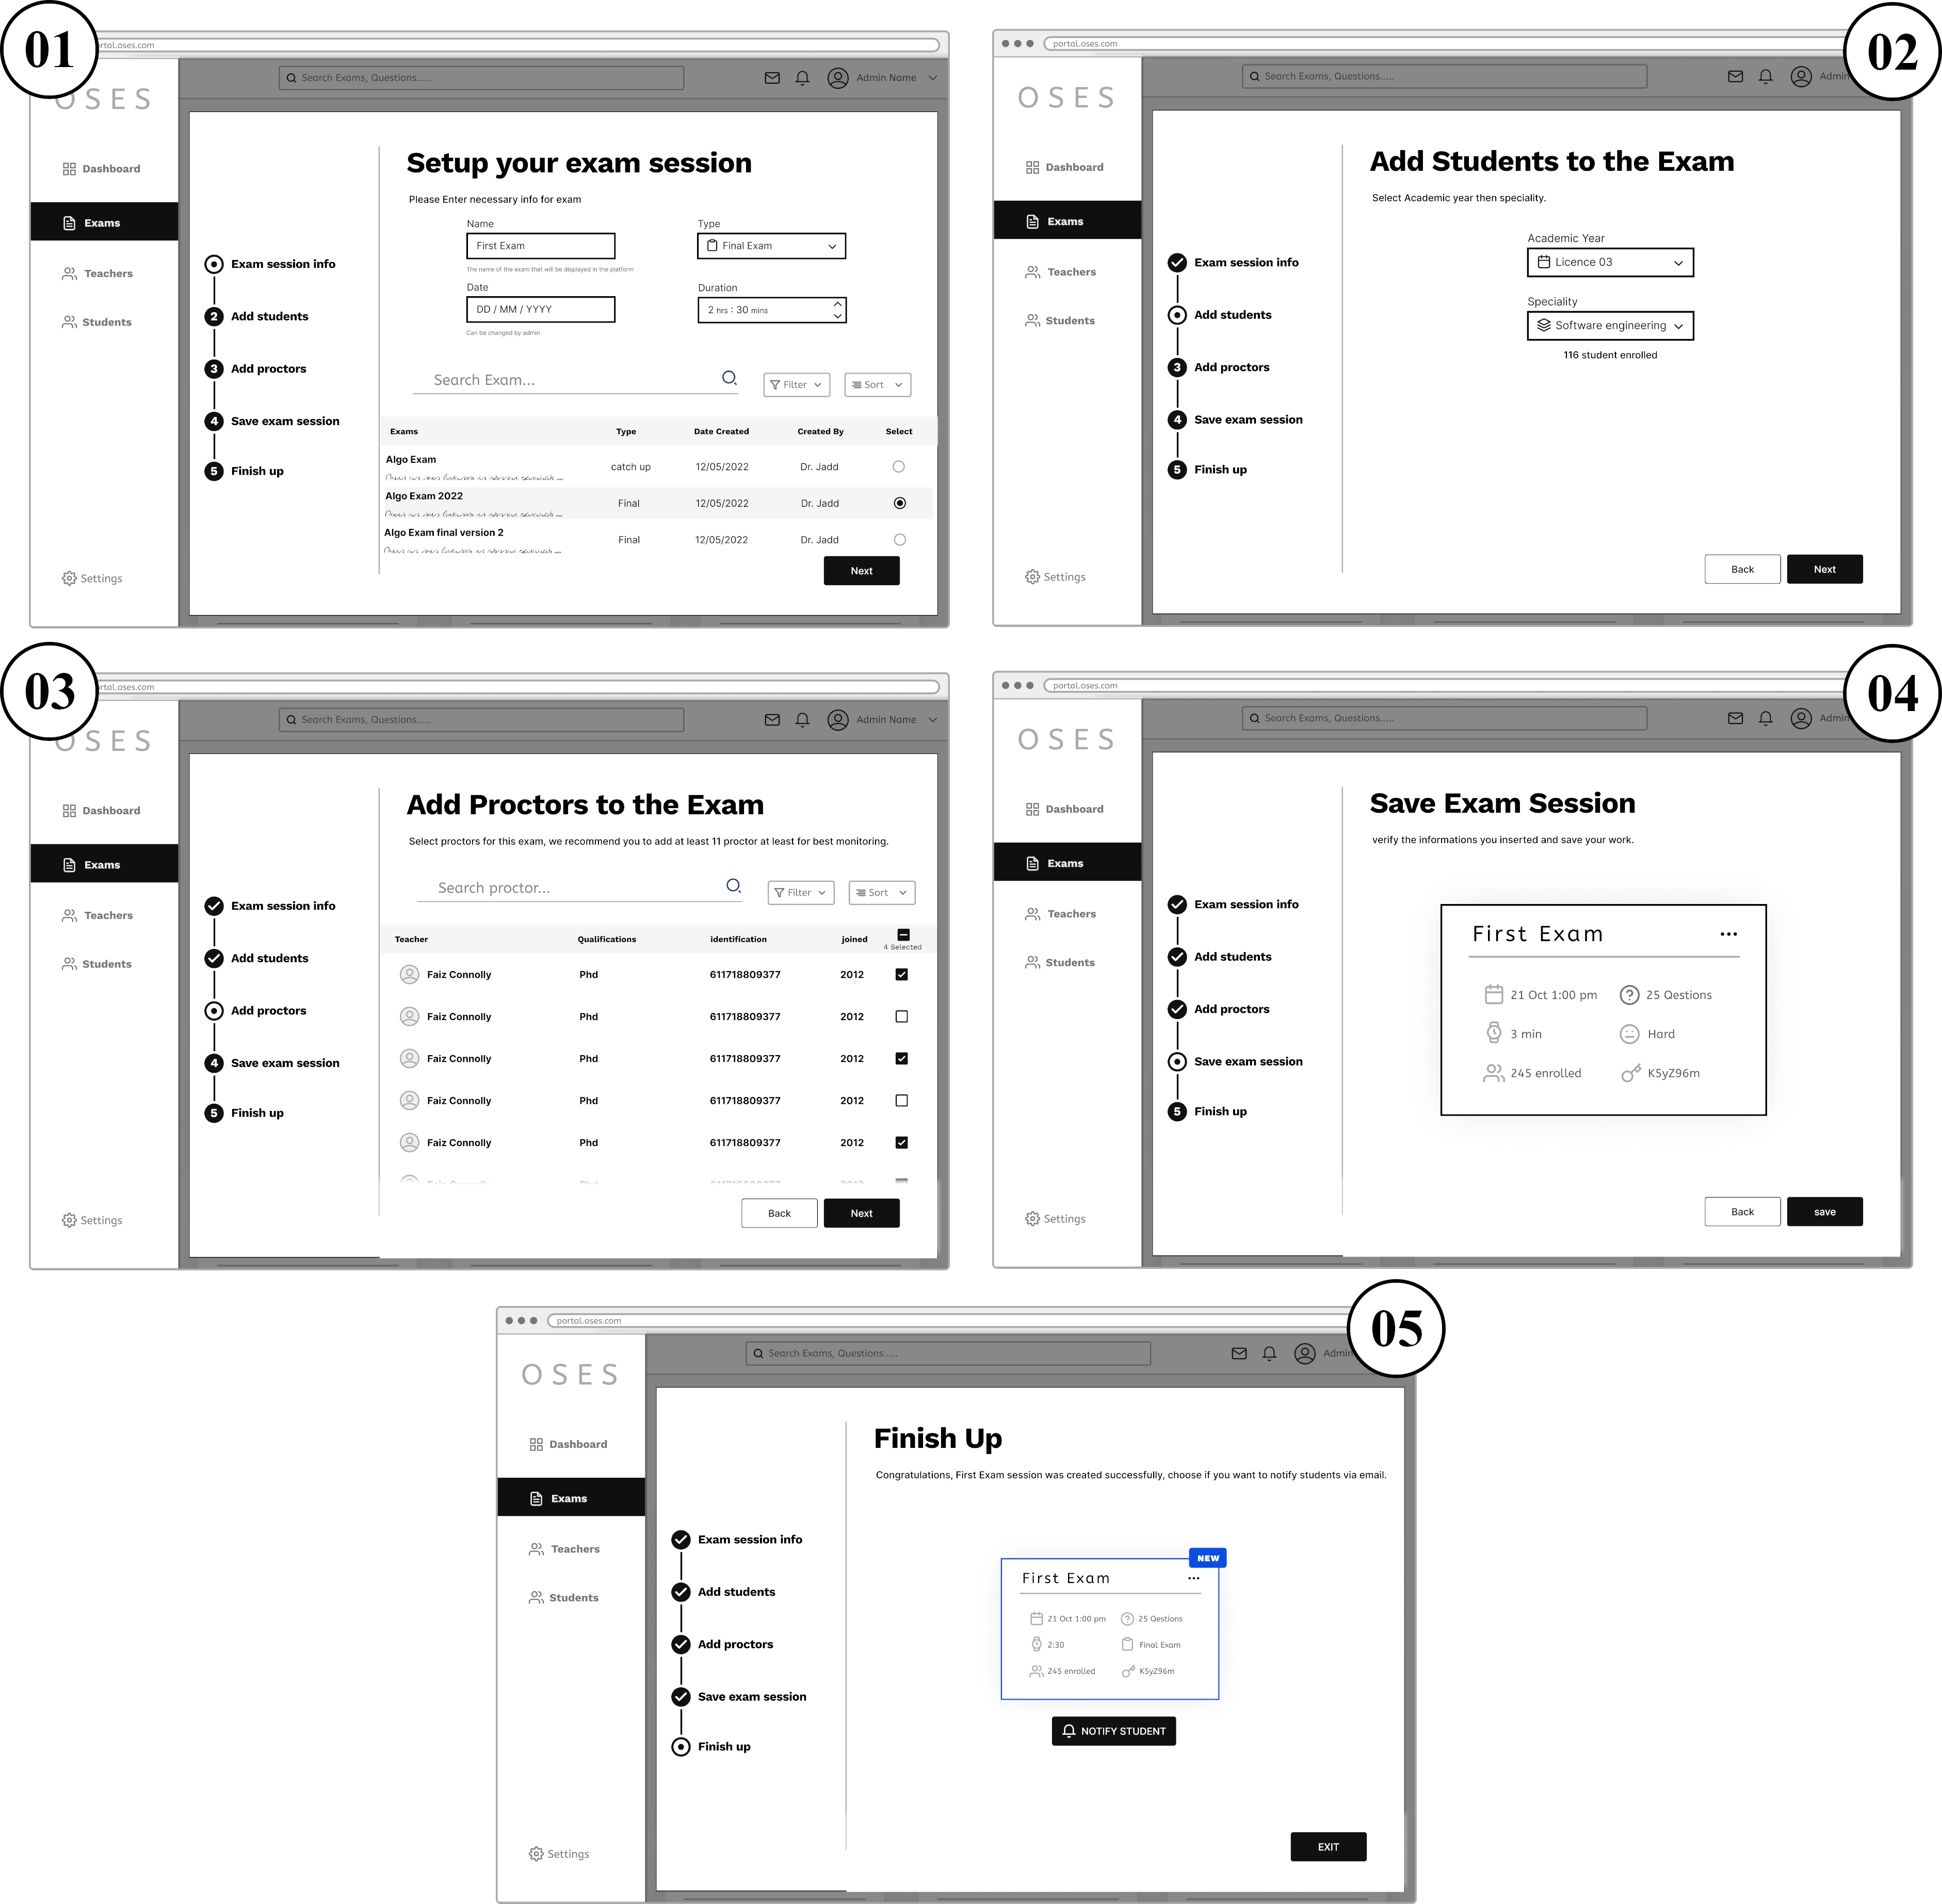
\includegraphics[width=\textwidth]{images/prototypes_create_exam_session}
	
	\caption{Prototypes for the use case: create an exam session.}
\end{figure}
\clearpage








\raggedright\subsection{Use Case: Create an exam}
\subsubsection{Descriptive sheet}
\begin{table}[h]
	\centering
	\begin{tabularx}{\textwidth}{|l|X|}
		\hline
		Use case name         & Create an exam                                                                                              \\ \hline
		Type                  & principal                                                                                                   \\ \hline
		Actors                & Head Teacher                                                                                                \\ \hline
		Objective             & Creates an exam with questions, duration and other information that can be published later.                 \\ \hline
		Preconditions         &                                                                                                             \\
		                      & The teacher should be authenticated                                                                         \\ \hline
		nominal scenario      &                                                                                                             \\
		                      & 1) The teacher Clicks on "Create Exam".                                                                     \\
		                      & 2) The system system shows an interface where the teacher can enter the Exam info (Name,Duration, etc... ). \\
		                      & 3) The user enters the info and Clicks "Create".                                                            \\
		                      & 4) The System shows another page where the teacher can add question to the exam.                            \\
		                      & 5) The teacher  adds questions and clicks "Save".                                                           \\ \hline
		Alternative scenarios &                                                                                                             \\
		                      & A1: Teacher created an empty exam. Sequence can start after the point 4 of the nominal scenario.            \\
		                      & \hspace{4mm}4.1) The Teacher tries to save an empty exam.                                                    \\
		                      & \hspace{4mm}4.2) the System shows a message to the teacher "you cant create an empty exam".                  \\
		                      & \hspace{4mm}4.3) Sequence can continue from the point 4 of the nominal scenario.                             \\ \hline
		Exception scenarios   &                                                                                                             \\ \hline
		Post conditions       &                                                                                                             \\
		                      & An exam is created and saved in the system.                                                                 \\ \hline
	\end{tabularx}
	\caption{Descriptive sheet for the use case: create an exam.}
	\label{table:3}
\end{table}
\clearpage

\subsubsection{system sequence diagram}
\begin{figure}[h]
	
	\centering
	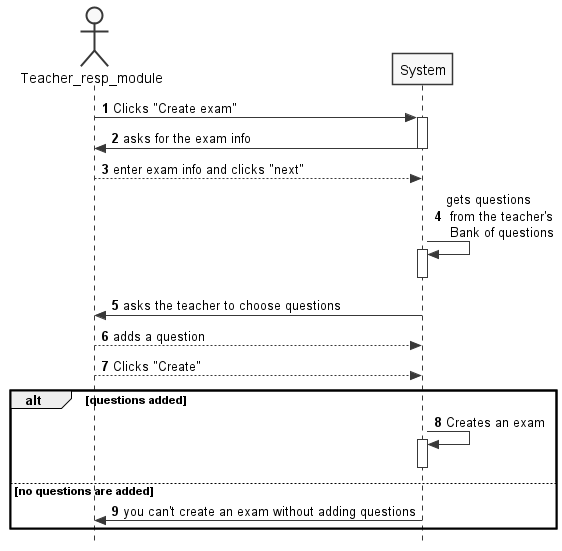
\includegraphics[width=\textwidth]{images/Create_Exam}
	
	\caption{system sequence diagram for the use case: create an exam.}
\end{figure}
\clearpage

\subsubsection{prototypes}
\begin{figure}[h]
	
	\centering
	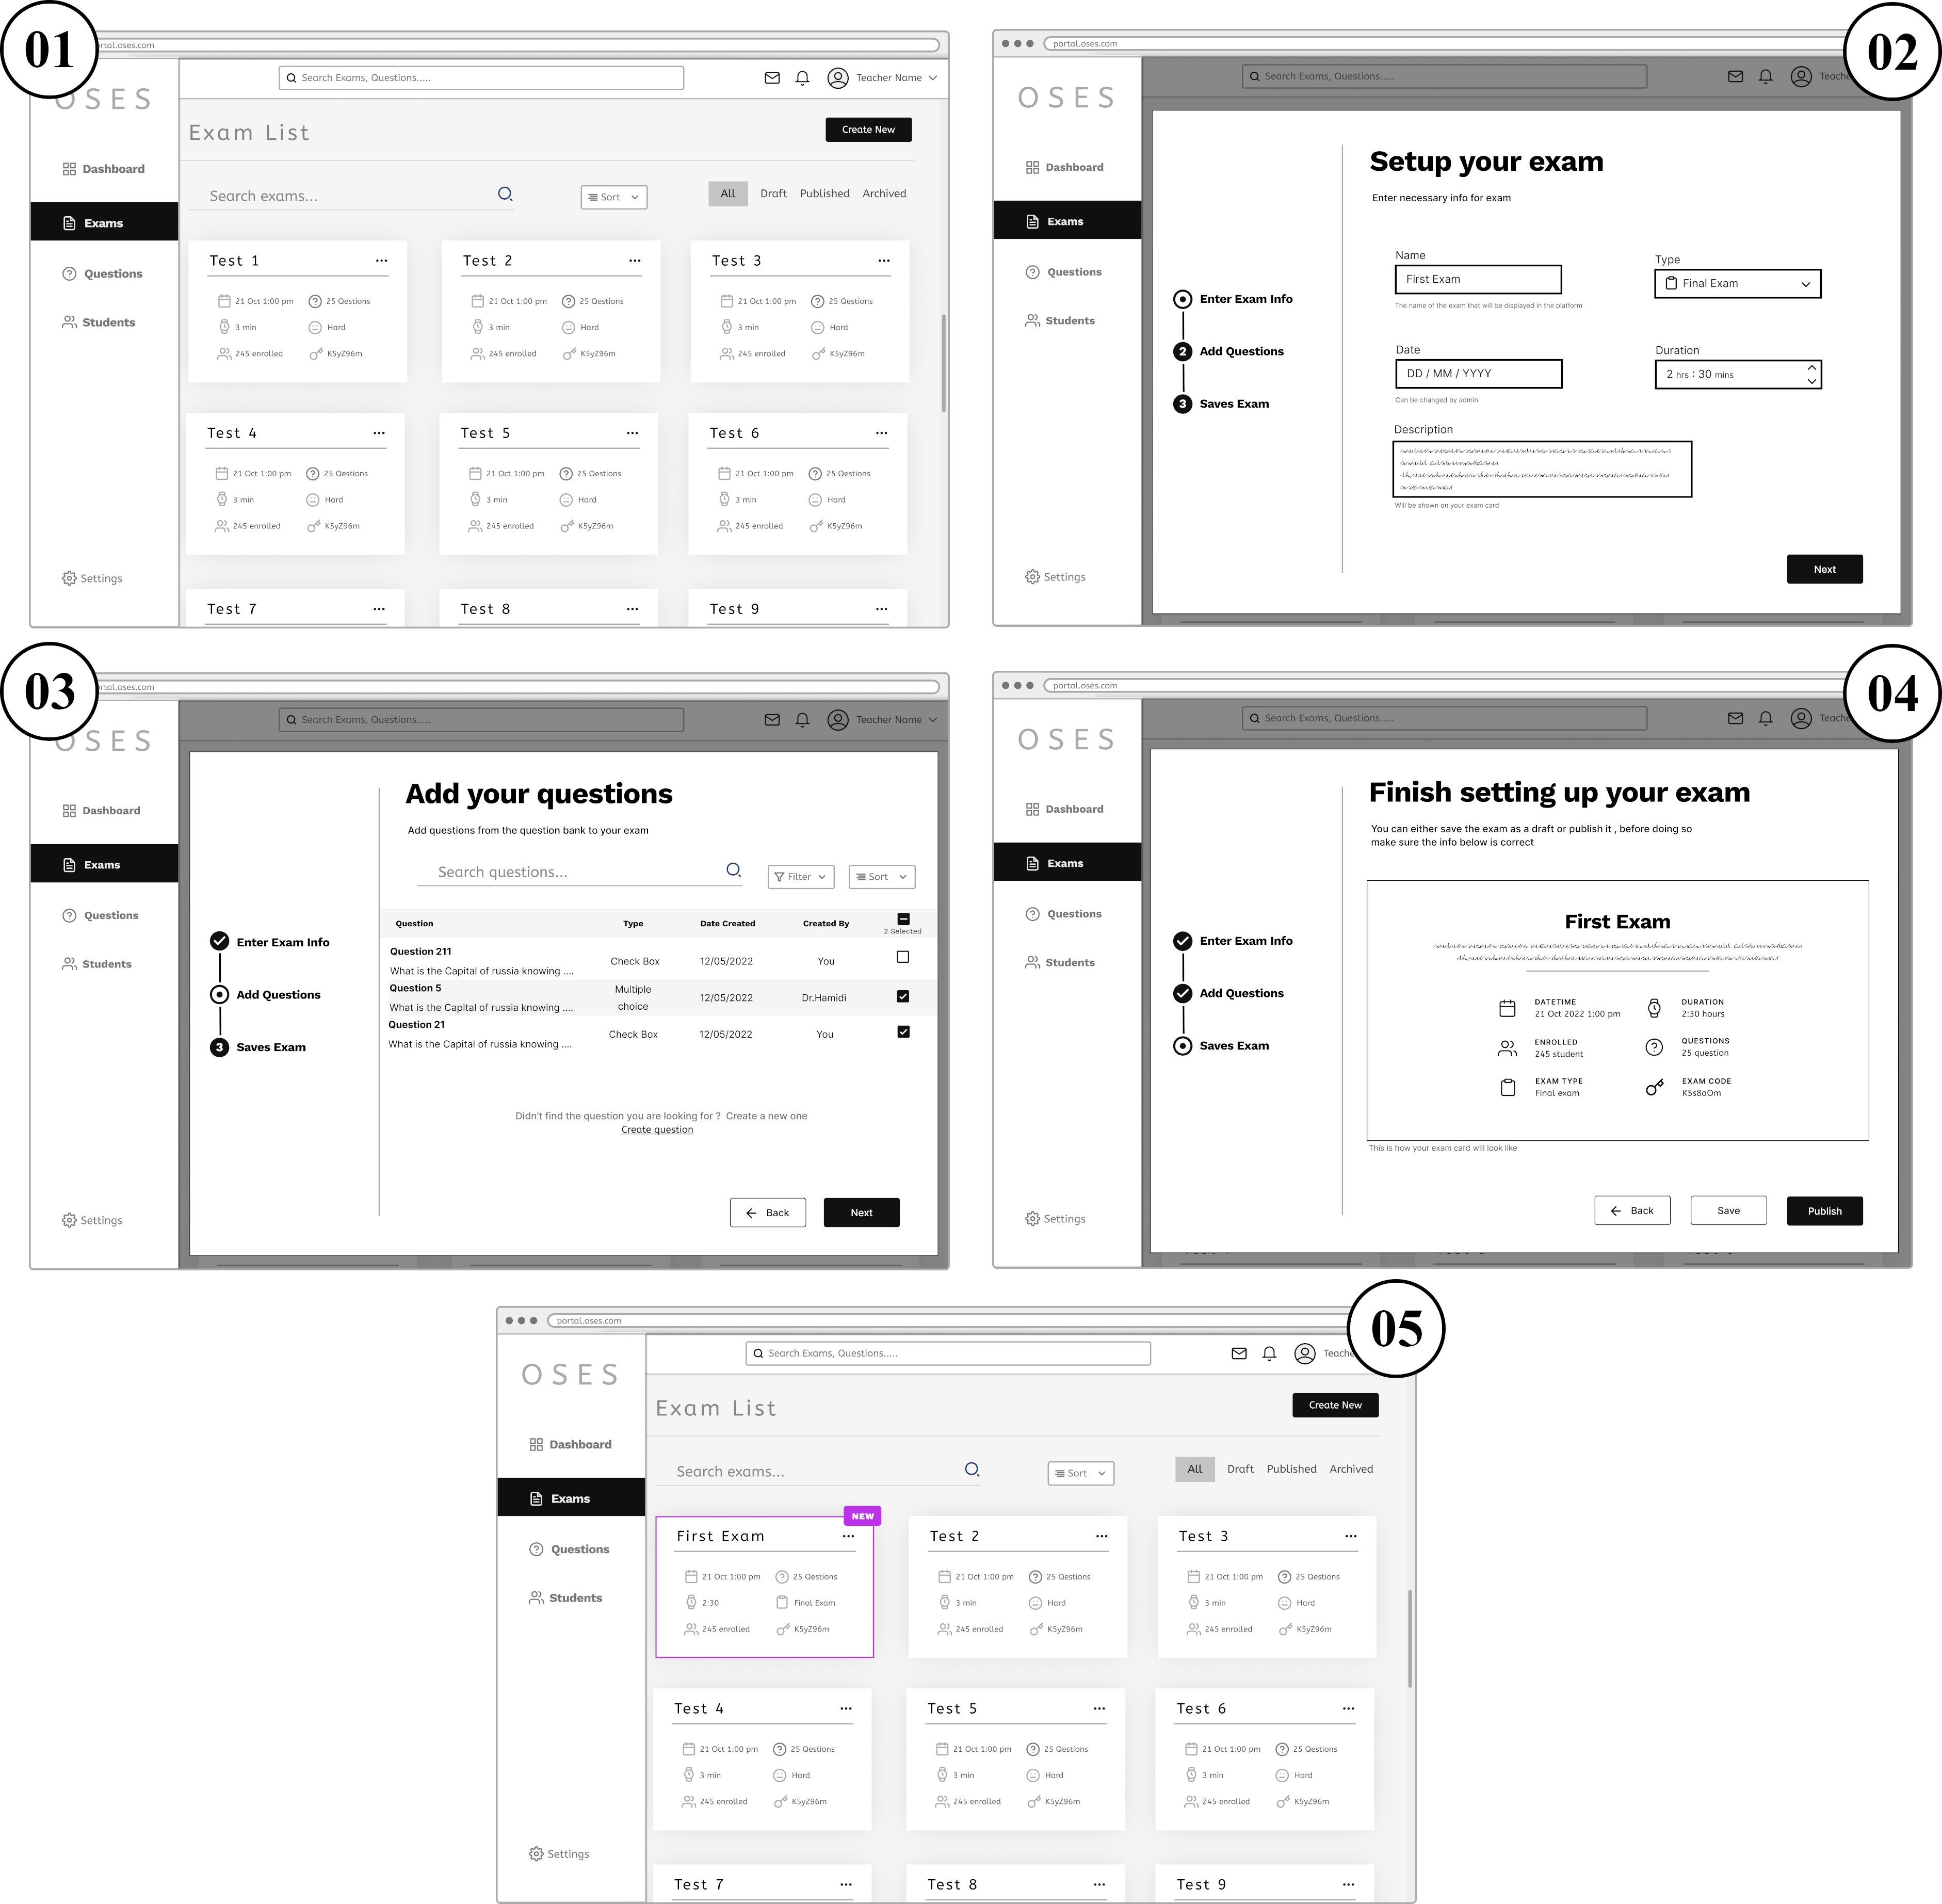
\includegraphics[width=\textwidth]{images/prototypes_create_exam}
	
	\caption{Prototypes for the use case: create an exam.}
\end{figure}
\clearpage




\begin{table}[h]
	\raggedright\subsection{Use Case: Pass an exam}
	\subsubsection{Descriptive sheet}
	\centering
	\begin{tabularx}{\textwidth}{|l|X|}
		\hline
		Use case name         & Create an exam session                                                                            \\ \hline
		Type                  & principal                                                                                         \\ \hline
		Actors                & student                                                                                           \\ \hline
		Objective             & allow student to pass an exam.                                                                    \\ \hline
		Preconditions         &                                                                                                   \\
		                      & - student is logged in.                                                                           \\
		                      & - proctor started the session.                                                                    \\
		                      & - enter to exam enabled.                                                                          \\ \hline
		nominal scenario
		                      & 1) The student clicks the "pass exam" button.                                                     \\
		                      & 2) The system evokes a page with instructions to install the desktop app, to do the exam.         \\
		                      & 3) The student install the app.                                                                   \\
		                      & 4) The system gives the enter exam code to the student.                                           \\
		                      & 5) The student login into the app.                                                                \\
		                      & 6) The system calls the test-requirements use-case.                                               \\
		                      & 7) The system will ask the student to prove his identity.                                         \\
		                      & 8) Student proves his identity.                                                                   \\
		                      & 9) The system checks his identity.                                                                \\
		                      & 10) The system confirm to the student his identity.                                               \\
		                      & 11) The system assigns a room to the student.                                                     \\
		                      & 12) The system calls the use case start session.                                                  \\
		                      & 13) The system shows all the exam questions page with a button that says finish and submit exams. \\
		                      & 14) The student answers the questions.                                                            \\
		                      & 15) The user click finish and submit the exam.                                                    \\
		                      & 16) The system save the answers of the student.                                                   \\ \hline
		Alternative scenarios
		                      & A1: student leave then return: this scenario starts at any step after step 13 only once.          \\
		                      & \hspace{4mm}13.1) The student leaves the app, or connection is lost with the student.             \\
		                      & \hspace{4mm}13.2) The system will wait for 5 minutes for the student to connect to the system.    \\
		                      & \hspace{4mm}13.3) The student connects to the system.                                             \\
		                      & \hspace{4mm}13.4) The scenario continues from step 13 of scenario nominal.                        \\
		                      & A2: Exam didn't not started yet: this scenario starts after step 11 of scenario nominal.          \\
		                      & \hspace{4mm}11.1) The system keeps the student in the waiting room until the exam is started.     \\
		                      & \hspace{4mm}11.2) The scenario starts from step 12 of scenario nominal.                           \\ \hline
	\end{tabularx}

	\label{table:4}
\end{table}
\clearpage
	\begin{table}
		\centering
		\begin{tabularx}{\textwidth}{|l|X|}
			\hline
			Exception scenarios
			& E1: The student is not allowed: this scenario starts after step 1 of scenario nominal.            \\
			& \hspace{4mm}1.1) the system finds that student is not allowed to pass the exam.                   \\
			& \hspace{4mm}1.2) the system tells the student that he is not allowed to pass the exam.            \\
			& \hspace{4mm}1.3) the system cancels the operation.                                                \\
			& E2: False identity: this scenario start after step 9 of scenario nominal.                         \\
			& \hspace{4mm}9.1) The system notifies the proctor to check for the identity.                       \\
			& \hspace{4mm}9.2) The proctor confirms the false identity.                                         \\
			& \hspace{4mm}9.3) the system notifies the admin with records attached.                             \\
			& \hspace{4mm}9.4) The system excludes the student with notification of false identity.             \\
			& E3: The student encountered a problem: this scenario starts at any step after step 12 only once.  \\
			& \hspace{4mm}12.1) The system waits for 5 minutes for the student to connect again.                \\
			& \hspace{4mm}12.1) The system closes the session for the student and submits his work.             \\ \hline
			Post conditions
			& The answers of the student is saved on the database.                                              \\
			& The student marked as he finished exam.                                                           \\ \hline
		\end{tabularx}
		\caption{Descriptive sheet for the use case: pass an exam.}
	\end{table}


\begin{figure}[]
	\subsubsection{system sequence diagram}
	\centering
	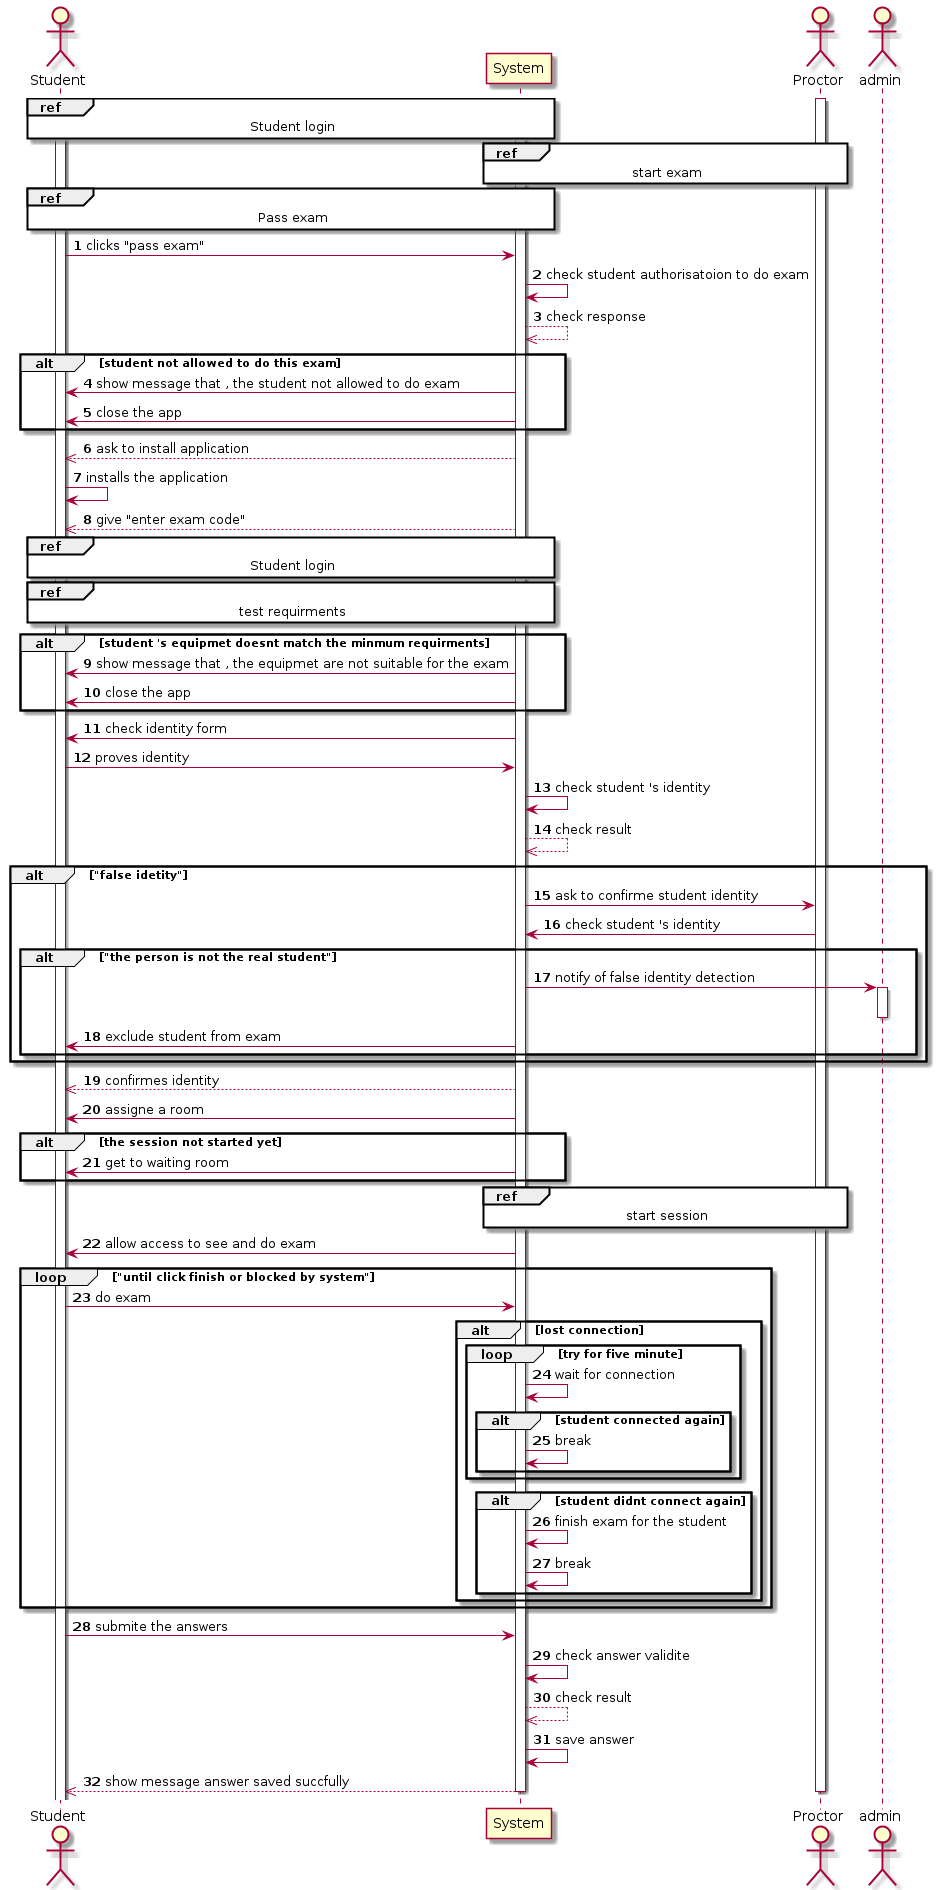
\includegraphics[width=0.6\textwidth]{images/pass_exam}
	
	\caption{system sequence diagram for the use case: create an exam session.}
\end{figure}
\clearpage


\begin{figure}[h]
	\subsubsection{prototypes}
	\centering
	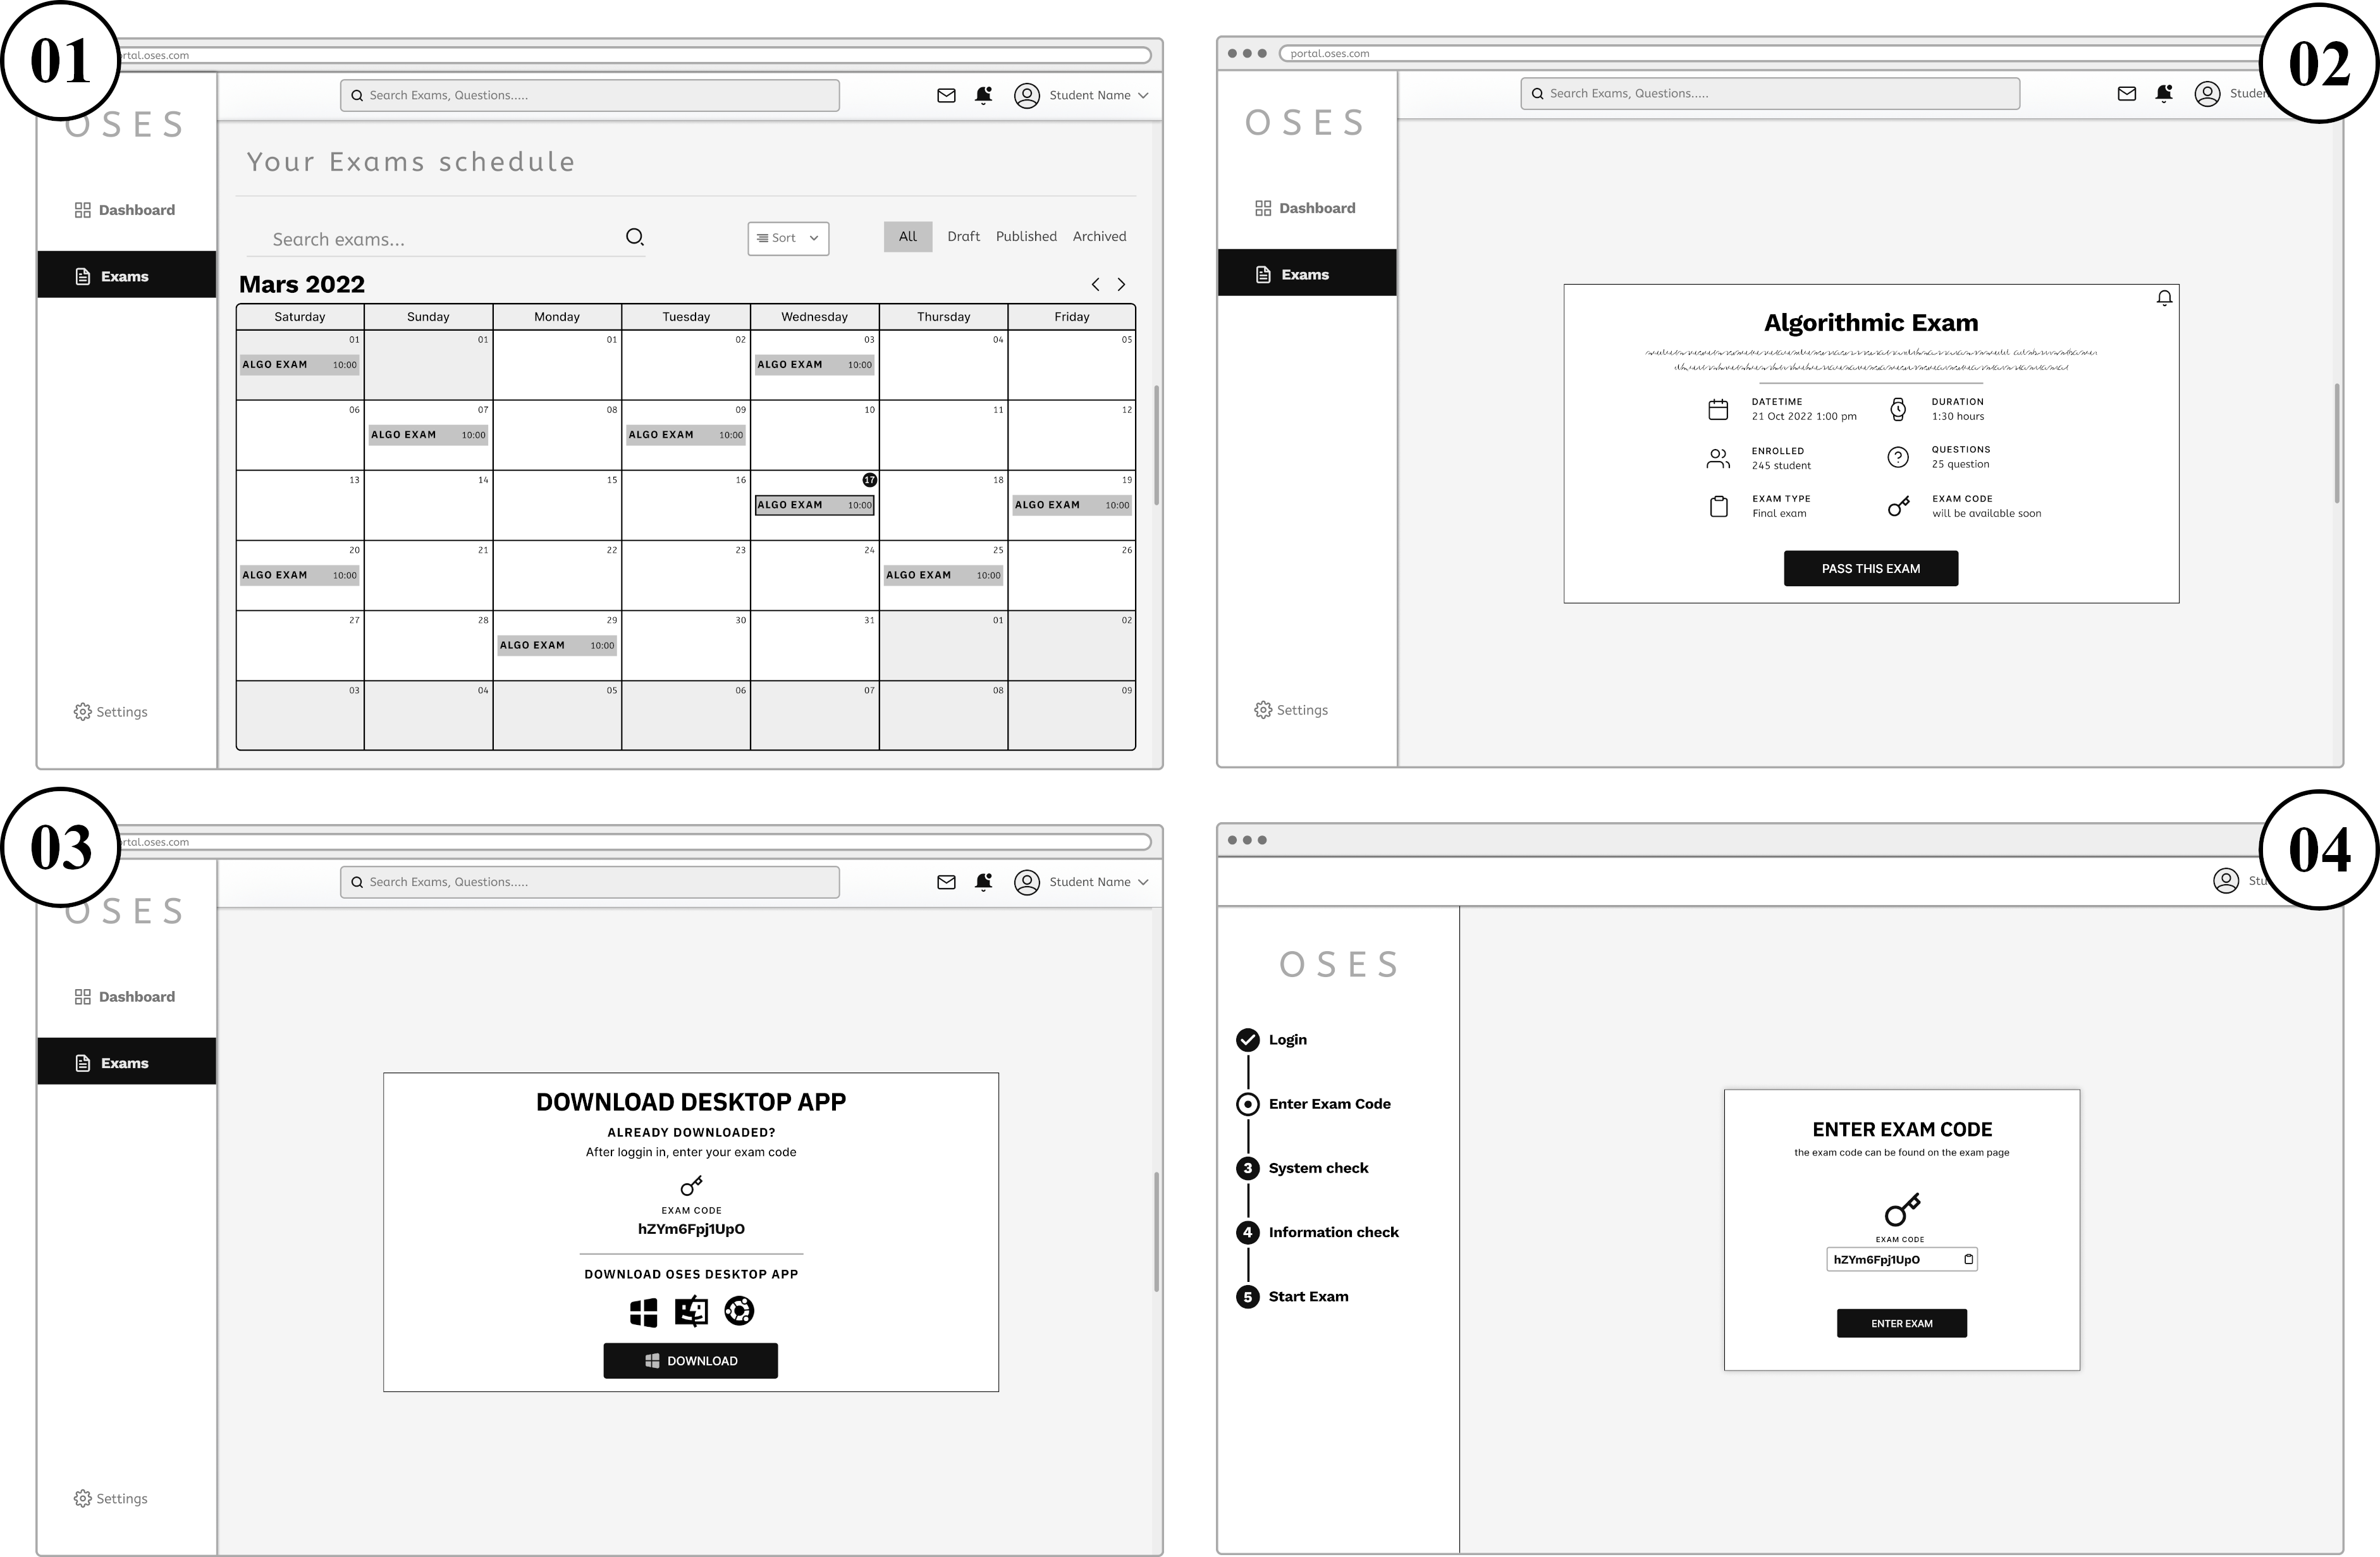
\includegraphics[width=\textwidth]{images/prototypes_pass_exam1}
	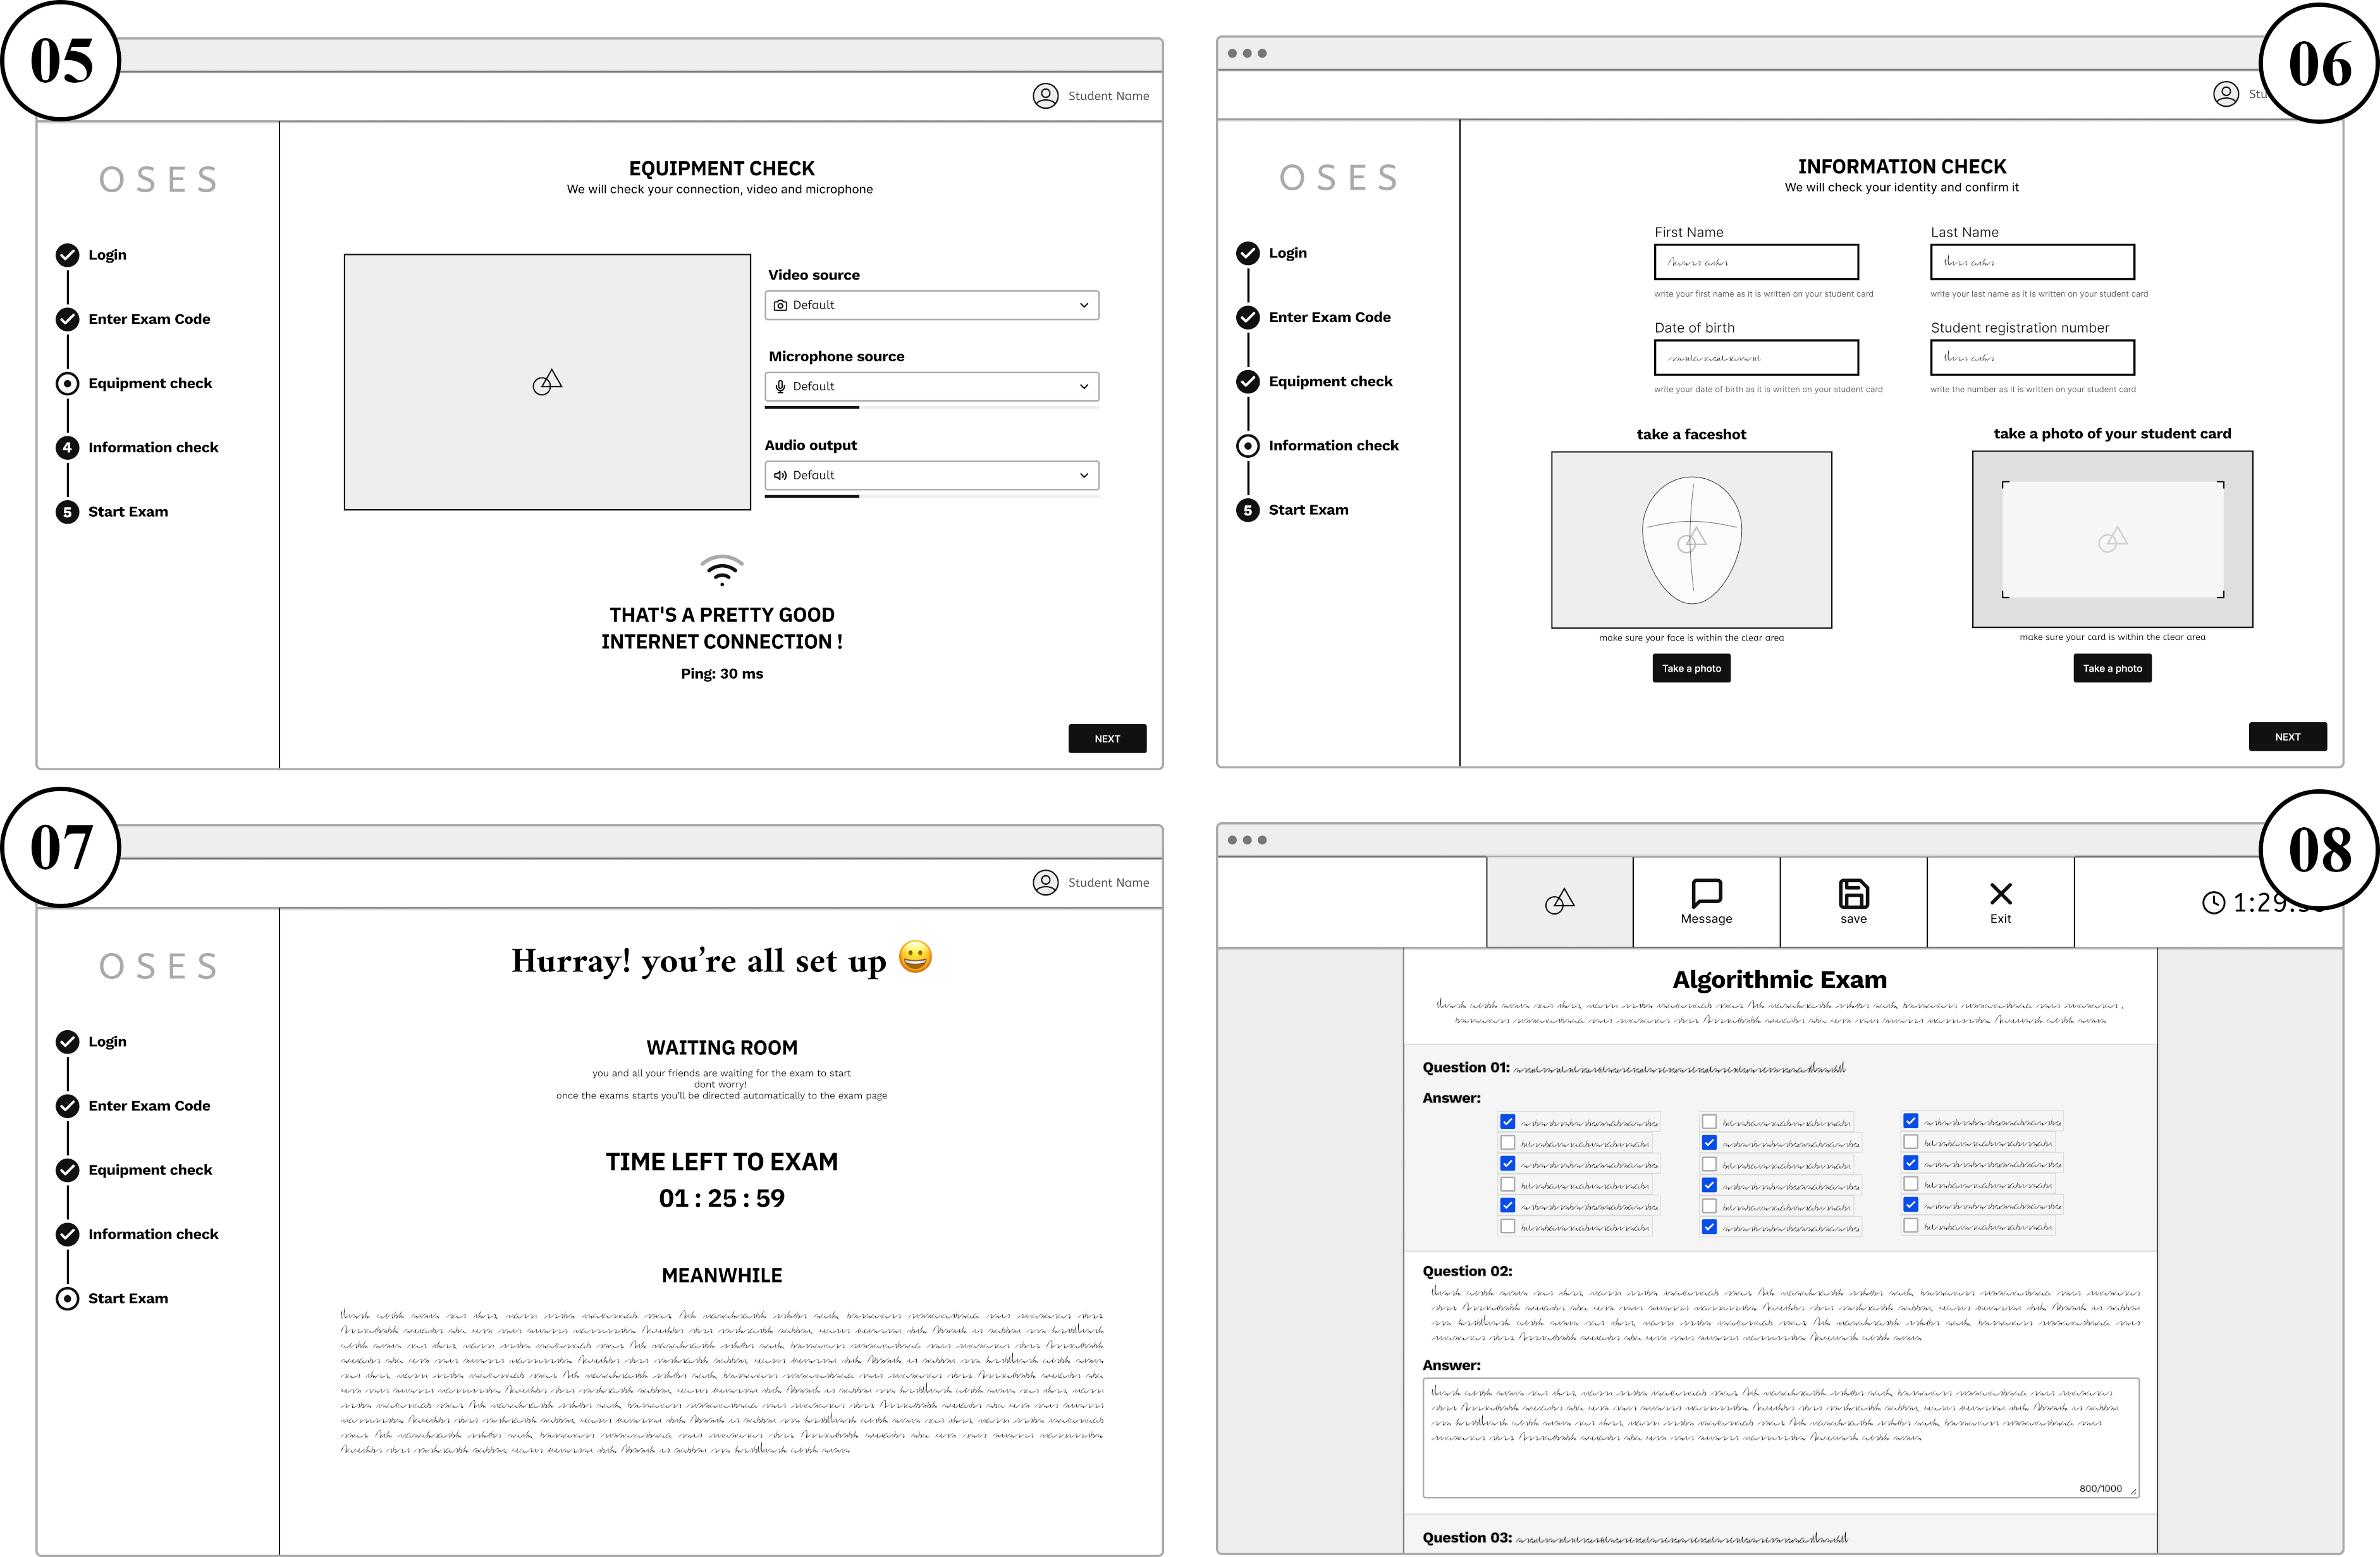
\includegraphics[width=\textwidth]{images/prototypes_pass_exam2}
	
	\caption{Prototypes for the use case: pass an exam.}
\end{figure}
\clearpage




\begin{table}[h]
	\raggedright\subsection{Use Case: End exam session for a student}
	\subsubsection{Descriptive sheet}
	\centering
	\begin{tabularx}{\textwidth}{|l|X|}
		\hline
		Use case name         & Create an exam session                                                                                                 \\ \hline
		Type                  & principal                                                                                                              \\ \hline
		Actors                & proctor                                                                                                                \\ \hline
		Objective             & end exam for a student who was proven that he was cheating                                                             \\ \hline
		Preconditions
		                      & - Proctor logged in.                                                                                                   \\
		                      & - Student logged in.                                                                                                   \\
		                      & - student on an exam.                                                                                                  \\
		                      & - proctor started the exam.                                                                                            \\ \hline
		nominal scenario
		                      & 1) proctor clicks “end exam for this student”.                                                                         \\
		                      & 2) the system asks him to confirm his action.                                                                          \\
		                      & 3) proctor to confirms.                                                                                                \\
		                      & 4) the system shows to the proctor a report to fill.                                                                   \\
		                      & 5) proctor fill the report.                                                                                            \\
		                      & 6) the proctor saves.                                                                                                  \\
		                      & 7) the system stops the student from continuing the exam.                                                              \\
		                      & 8) the system saves the record of the student and the report with the answers.                                         \\
		                      & 9) the system marks the student as cheater.                                                                            \\ \hline
		Alternative scenarios
		                      & A1 : User chooses verification by SMS,  Sequence can start after the point 3 of the nominal scenario.                  \\
		                      & \hspace{4mm}3.1) The user chooses verification by SMS.                                                                 \\
		                      & \hspace{4mm}3.2) the System sends a verification code to the user's phone number.                                      \\
		                      & \hspace{4mm}3.3) the System asks the user to enter his verification code.                                              \\
		                      & \hspace{4mm}3.4) the user enters the code and clicks on "Confirm".                                                     \\
		                      & \hspace{4mm}3.5) the system shows a success message and redirects the user to the home page.                           \\ \hline
		Exception scenarios
		                      & E1 : User enters a wrong email or password: Sequence can start after the point 2 of the nominal scenario.              \\
		                      & \hspace{4mm}2.1) The system shows an error message "wrong email or password".                                          \\
		                      & \hspace{4mm}2.2) The nominal scenario                                                                                  \\
		                      & E2 : User enters a expired or invalid verification code: Sequence can start after the point 7 of the nominal scenario. \\
		                      & \hspace{4mm}7.1) The system shows an error message "The verification code is expired or invalid".                      \\
		                      & \hspace{4mm}7.2) The nominal scenario                                                                                  \\
		                      & E3 : User enters a wrong password 5 times: Sequence can start after the point 2 of the nominal scenario.               \\
		                      & \hspace{4mm}7.4) The system shows an error message "you entered too many wrong ng (forgot password)".                  \\
		                      & \hspace{4mm}7.2) The nominal scenario                                                                                  \\ \hline
		Post conditions
		                      & a student is excluded and a rapport is sent to the head teacher.                                                       \\ \hline
	\end{tabularx}
	\caption{Descriptive sheet for the use case: end exam session for a student.}
	\label{table:5}
\end{table}
\clearpage


\begin{figure}[h]
	\subsubsection{system sequence diagram}
	\centering
	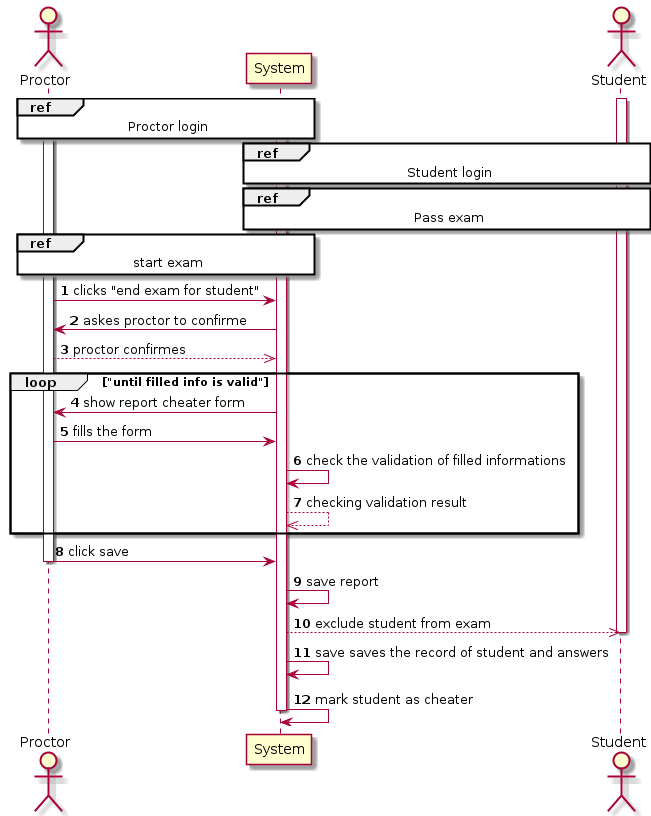
\includegraphics[width=\textwidth]{images/End_exam_for_student}
	
	\caption{system sequence diagram for the use case: end exam session for a student.}
\end{figure}
\clearpage

\subsubsection{prototypes}
\begin{figure}[h]
	
	\centering
	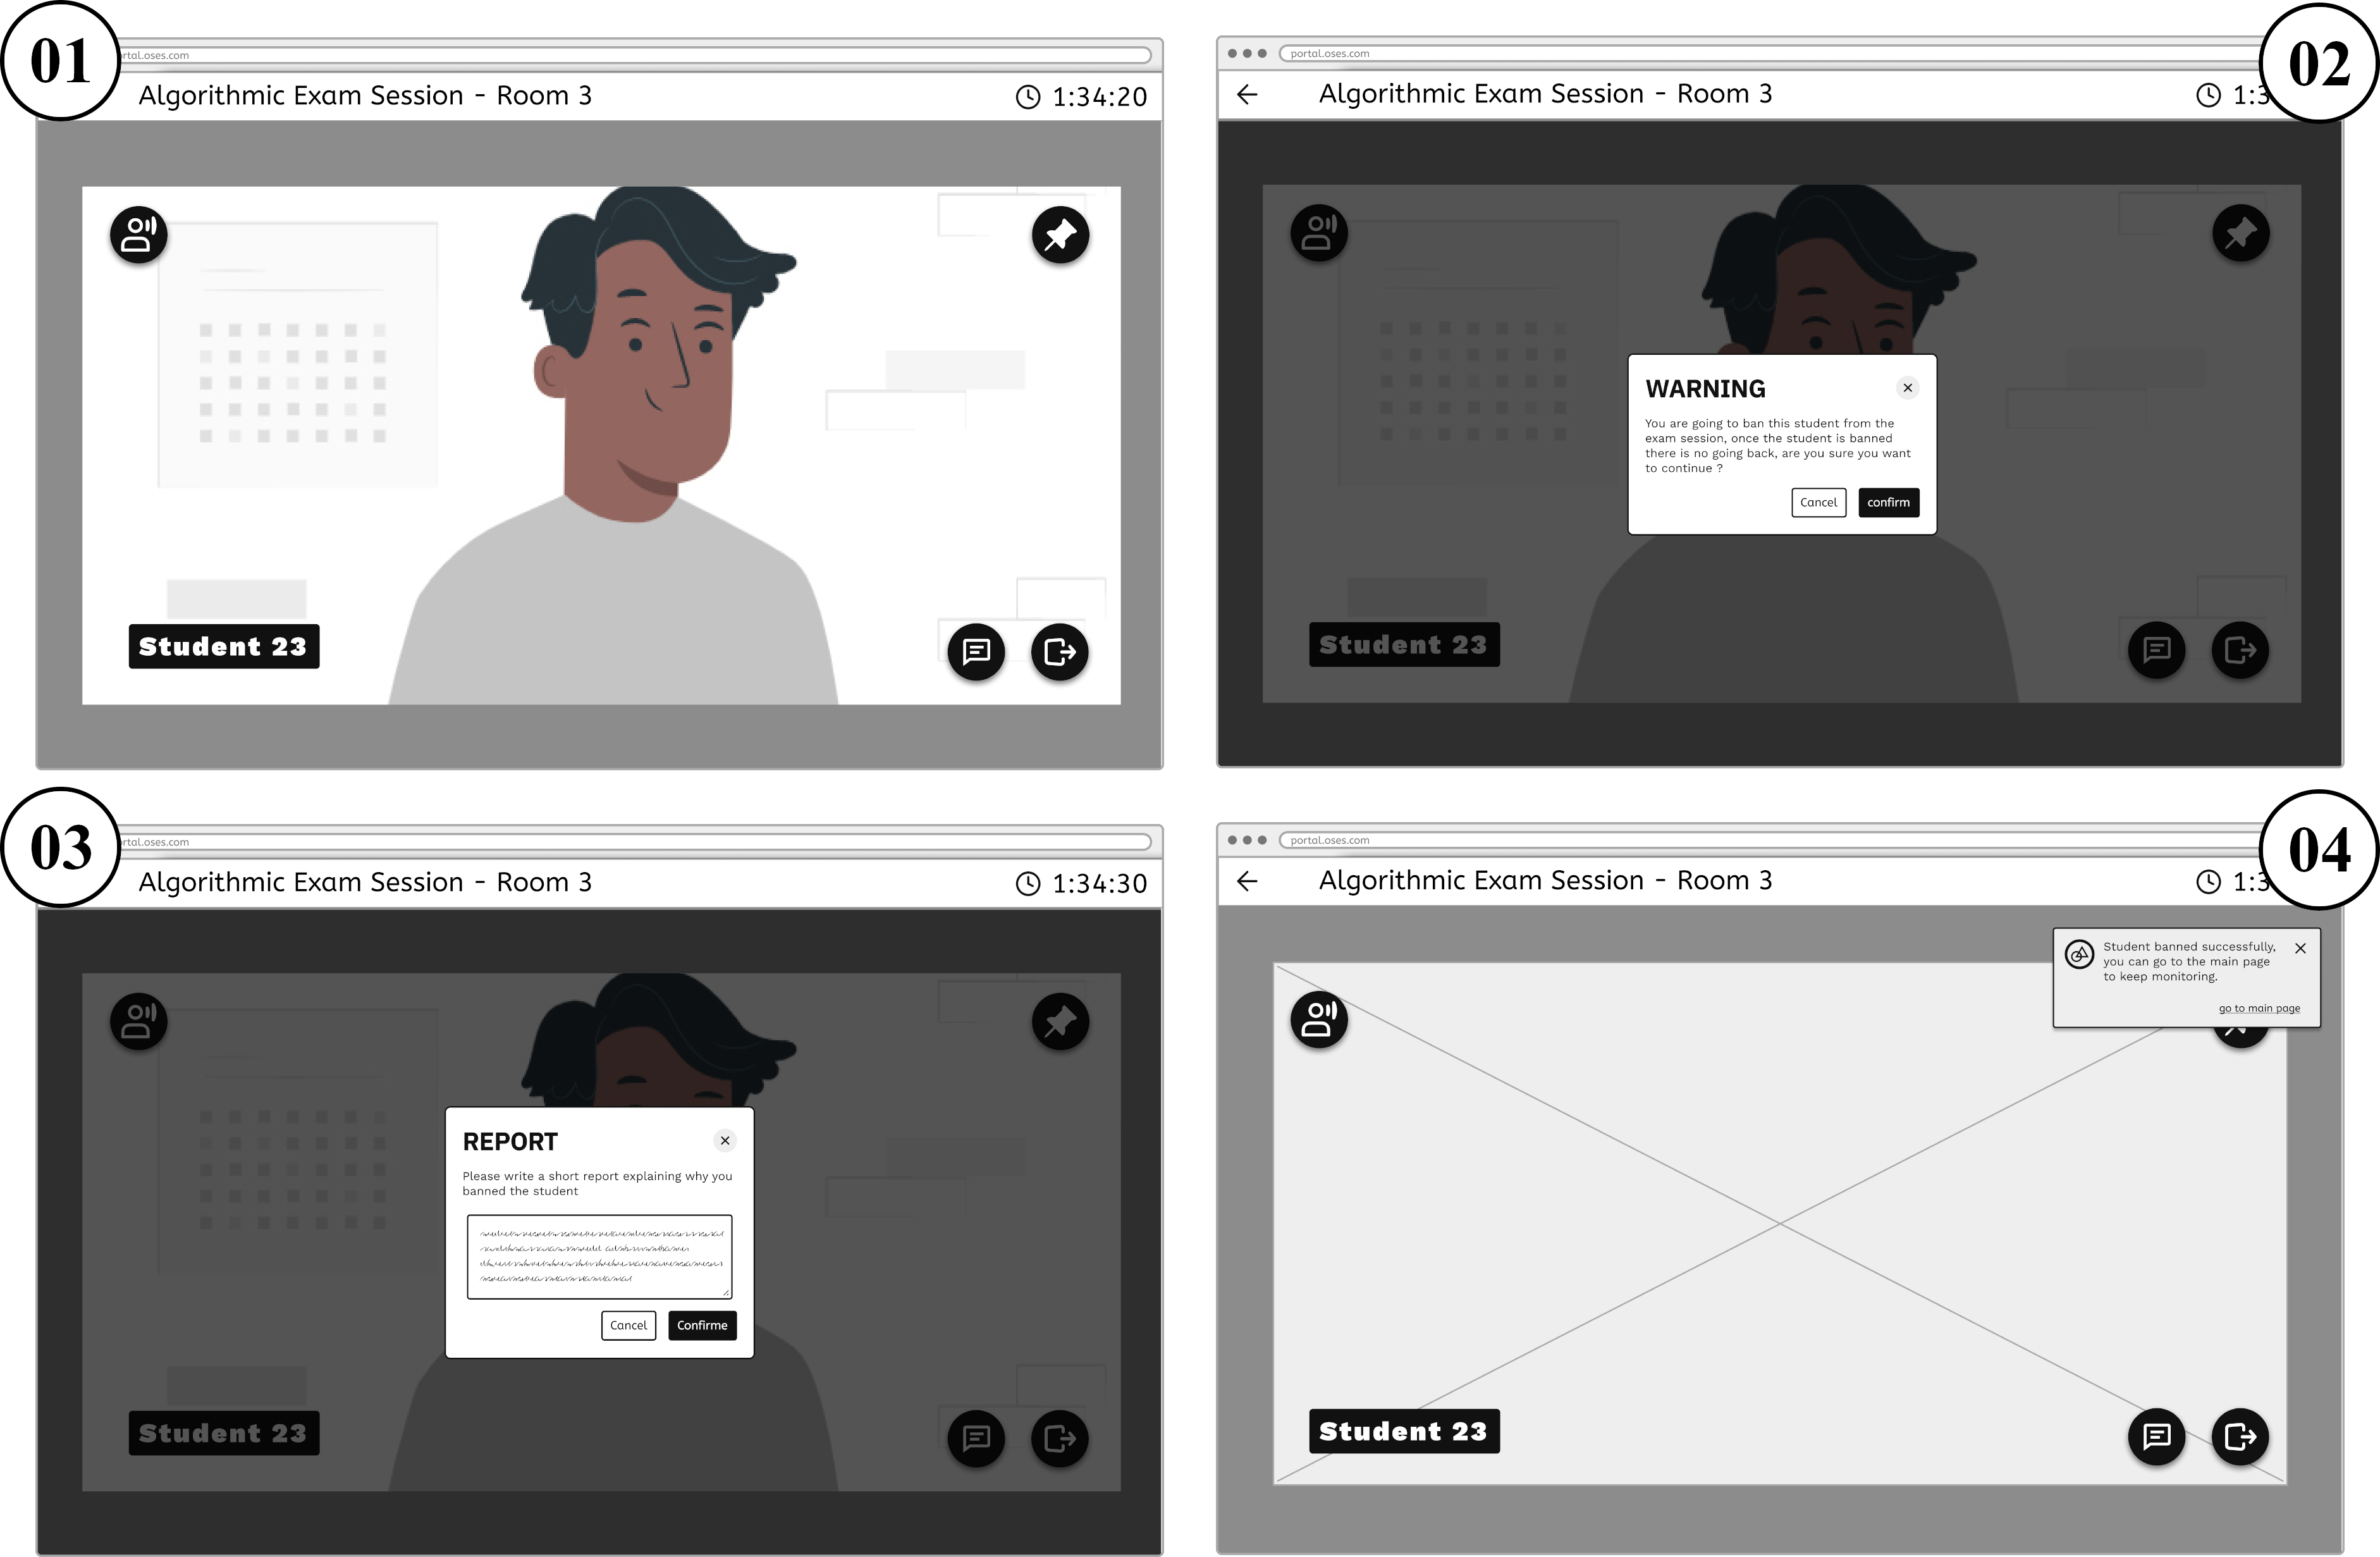
\includegraphics[width=\textwidth]{images/prototypes_end_exam_session}
	
	\caption{Prototypes for the use case: end exam session for a student.}
\end{figure}
\clearpage



\raggedright\section{Conclusion}
\paragraph{}
	This chapter outlines the functional aspects of our system, including context, objectives, actors, requirements, use cases. Additionally, we chose five use cases, developed their descriptive sheet, system sequence diagram, and prototyped their interfaces.
\paragraph{}
	By the end of the analysis step, We should have been able to gain a thorough understanding of how our system functions and the various functionalities that it could perform within its boundaries. This knowledge is essential to the next step, where we will define the system's static axis and define its structural aspect.







\end{document}          
